% !TEX root = atlas_latex.tex

%-------------------------------------------------------------------------------
% Body of the guide to the use of the ATLAS LaTeX package
%-------------------------------------------------------------------------------
\section{Introduction}
\label{sec:intro}
%-------------------------------------------------------------------------------

This collection of ATLAS \LaTeX\ templates, style files and documentation
can be used for papers, preprints and notes, both public and internal. 
All necessary files are collected in a single package called \Package{atlaslatex}.
The package is available from the web pages of the Publication Committee~\cite{pubcom} and from 
Git~\cite{pubcom-git}.

\ADOCnew{09-00-00} The package should work for \TeX\ Live versions from 2013 onwards.
\ADOCnew{II-JJ-KK} indicates the version number of ATLAS \LaTeX\ when new features are added.
\ADOCold{II-J-KK} indicates the version number when a feature is removed or made obsolete.

The collection replaces and improves on the previous packages.
In particular it supersedes:
\begin{itemize}\setlength{\parskip}{0pt}\setlength{\itemsep}{0pt}
\item \texttt{atlasnote-00-04-05}
\item \texttt{atlascover-00-00-11}
\item \texttt{atlaspreprint-00-00-05}
\item \texttt{atlasbib-00-00-04}
\end{itemize}
\Cref{sec:oldnote} summarises the changes that have been made and
how you can adapt your documents to use the new package.
\Cref{sec:oldcover} summarises the changes to the cover macros.

The package includes the \Package{atlasdoc} class, useful style files
and documentation of the package.
The package also defines a standard ATLAS style for papers.
This style should be used for paper drafts and for submission to the arXiv and the journal.
This option is the default. Add the option \Option{atlasstyle=false} to the \Package{atlasdoc} class if you do not want to use this style.
The documentation is provided as both PDF files and \LaTeX\ documents
that should provide examples of how to use the package and how to write
good \LaTeX.

The design principle is that you have a main document and 
the style files and \Package{atlasdoc} class are in a subdirectory \File{latex}.
The logos that are needed are kept in a \File{logos} directory.
These subdirectories can of course be links to a centrally maintained \texttt{latex} directory.
See below and \cref{sec:texmf} for how to proceed if you want to use and/or install
the package in a central place.

The usual procedure is that for each document that you create,
you first unpack the latest version of \Package{atlaslatex} and
then create your main document in the top-level directory.
This structure means that it is easier to update the style files if a new version of
\Package{atlaslatex} is released. 
Each document can then be independent of the \Package{atlaslatex} release.

%------------------------------------------------------------------------------
\section{Getting started}
%------------------------------------------------------------------------------

To create a new document you can issue one of the commands:
%
\begin{bashlisting}
make newpaper [BASENAME=mydocument]
make newnote [BASENAME=mydocument]
\end{bashlisting}
depending on whether you want to write a paper/CONF Note/Pub Note draft or
an ATLAS note draft.
%
The command copies \File{atlas-paper.tex} or \File{atlas-note.tex} and
\File{atlas-paper-metadata.tex} or \File{atlas-note-metadata.tex}
to \File{mydocument.tex} and \File{mydocument-metadata.tex}.%
\footnote{The \File{Makefile} should work for regular Linux and MacOSX distributions.
For Windows, you probably have to execute the tasks in the \File{Makefile} by hand.}
The \texttt{make newpaper|newnote} command also creates empty files \File{mydocument-defs.sty} and \File{mydocument.bib}.
By default the document will be an ATLAS note draft.
Use \texttt{make newpaper} for an ATLAS paper draft (including CONF and PUB notes).
% If you want it to be a paper draft, add the option \Option{PAPER} to the document class.
Replace the option \Option{PAPER} with \Option{CONF} or \Option{PUB} as appropriate.

\emph{\ADOCold{14.0.0} Setting the \texttt{TEXLIVE} variable in the \texttt{make} command
is obsolete and ignored.}
In the past, the selected \TeX\ Live version was set by passing the
\Option{texlive} option to the document class.
This is no longer necessary.

In the \File{Makefile} you should change the \texttt{BASENAME} to the name of your document.
You can then compile your document with the command: \texttt{make}.
You can try the command \texttt{make run\_pdflatex} instead,
which runs \texttt{pdflatex} etc. \ directly
instead of invokes \texttt{latexmk}, a Perl script that is cleverer than the \texttt{Makefile}.
You can also make this command the default.
Have a look at \File{Makefile} for other things you can adjust.

If you install \Package{atlaslatex} in a central directory such as \File{\$\{HOME\}/texmf} the basic command is one of:
%
\begin{bashlisting}
make newpapertexmf [BASENAME=mydocument]
make newnotetexmf [BASENAME=mydocument]
\end{bashlisting}
%
See \cref{sec:texmf} for more details.

In order to make a new document of book form like a TDR, use one of the commands:
%
\begin{bashlisting}
make newbook [BASENAME=mydocument]
make newbooktexmf [BASENAME=mydocument]
\end{bashlisting}
%
By default, this will pass the option \Option{BOOK} to \Package{atlasdoc}.
Use \verb|make newbooktexmf| for a book with \Package{atlaslatex} in a central directory.

Note that you have to specify the language of your document as an option in the
\Macro{documentclass} command. Typical settings are
\begin{itemize}
\item UKenglish (or british);
\item USenglish (or american).
\end{itemize}

\ADOCold{14.0.0} The default \TeX\ Live version used to be set to 2020.
This was the only option you had to adjust if you use different versions of \LaTeX.
A different method is now used to find out which version is being run,
% You should be able to always set a version lower than the one you have installed to maintain compatibility with older versions.
To test compatibility with arXiv, you should compile your document using
\TeX\ Live 2020 on \File{lxplus} or another machine that has this version.
%This will, among other things, automatically switch from the \Package{newtx} fonts to \Package{txfonts} if you
%are using the ATLAS preprint style.

\ADOCnew{01-07-00} You should include the command \Macro{maketitle} after your\\
\verb|\begin{document}| if you want the document title to be printed.

Add the option \Option{atlasstyle=false} to the \Macro{documentclass}
if you do not want to typeset your document in the ATLAS preprint style.


%------------------------------------------------------------------------------
\section{ATLAS \LaTeX\ and the Physics Office GitLab project}
%------------------------------------------------------------------------------

With the move of ATLAS software and documents to Git,
new opportunities are available to streamline the production of documents
and smooth the process of submitting them to arXiv and journals.
This project is called PO-GitLab in the following~\cite{atlas-PO-gitlab}.

In order for the new tools to work smoothly some file-naming conventions should be followed.
If the Physics Office set up the Git repository, the files should already have the correct names.
The conventions are documented on
\url{https://gitlab.cern.ch/atlas-physics-office/gitlab-integration/wikis/newproject}.
For paper drafts, in short:
\begin{itemize}
  \item the main file should have the name \File{GROUP-YEAR-NUM-PAPER.tex};
  \item the metadata file should have the name \File{GROUP-YEAR-NUM-PAPER-metadata.tex};
  \item the auxiliary material should be included in a file with the name \File{GROUP-YEAR-NUM-PAPER-auxmat.tex}
\end{itemize}

In addition:
\begin{itemize}
  \item figures must be included using the \Macro{includegraphics} command;
  \item new commands should be defined in the \File{GROUP-YEAR-NUM-PAPER-defs.sty} file.
\end{itemize}


%-------------------------------------------------------------------------------
\section{Title, author and document numbers}
\label{sec:metadata}
%-------------------------------------------------------------------------------

An ATLAS document usually collects a series of labels over time.
These include the reference code of the analysis, e.g.\ \texttt{BPHY-2013-04}, 
the ATLAS note number and the CERN preprint number.
In addition the abstract and title are needed on the front page of the document and also on various cover pages.
The editors of the document, the editorial board members and the contributors to the analysis
also need to be specified at some point.

While all this information can be collected in the main file of the document, 
it is probably better to put it all in a separate document.
By default this file is called \texttt{mydocument-metadata.tex}.

\ADOCnew{04-00-00} As the metadata needed for ATLAS notes and ATLAS papers are somewhat different,
separate templates are used.


%-------------------------------------------------------------------------------
\subsection{Authors and Contributors}
\label{sec:contribute}
%-------------------------------------------------------------------------------

You can include an author's ORCID using the \Macro{AtlasOrcid} macro:\\
\verb+\AtlasOrcid[0000-0002-03-9876]{John Postdoc}+.
This command will be used in the ATLAS Collaboration author lists.

The supporting documentation for an ATLAS note (not the paper draft) should contain a list of the contributors to the analysis.
A style file \Package{atlascontribute.sty} has been written to help with the creation of such a list.
The macros in the style file can also build the author list at the same time.
Two basic macros are used to add names to the author list and list of contributions:
\Macro{AtlasContributor} and \Macro{AtlasAuthorContributor}. 
The first macro adds a person to the list of contributors, while the second one also adds the person
to the author list. I assume that in almost all cases you will want to use \Macro{AtlasAuthorContributor}.
An optional argument can be added to \Macro{AtlasAuthorContributor}, which contains the author's ORCID.
The author's name becomes a link to the ORCID.
Typical commands are:
\begin{tcblisting}{listing only}
\AtlasAuthorContributor{Joe Student}{a}{fake background estimate.}
\AtlasAuthorContributor{Jane Student}{b}{top background estimate.}
\AtlasAuthorContributor[0000-0002-03-9876]{John Postdoc}{a}{editor of internal note.}
\AtlasContributor{Jo Helper}{useful contributions in a few places.}
\affil[a]{University of Nowhere}
\affil[b]{University of Somewhere}
\end{tcblisting}
If a person should be added to the author list, you also need to add an appropriate affiliation using the macro \Macro{affil}.
The optional argument is a letter or number that should also be given as the second argument to
\Macro{AtlasAuthorContributor}.

You can keep the list of authors and contributors separate
by using \Macro{author} for the authors and \Macro{AtlasContributor} for the contributors.
You print the list of contributors by giving the command \Macro{PrintAtlasContribute}.
Note that \Macro{PrintAtlasContribute} has an argument that gives the fraction of the line width
to be used for the name of the person.
The list should either be printed before the table of contents or after the conclusions
(i.e.\ where the Acknowledgements appear in a paper).

Note that the \Package{authblk} package assumes that you will also have affiliations for each author.
You can avoid them by using the syntax \verb|\author{[ ]{Author Name}}|.
Note that a space is needed in the optional argument.
This means that a space appears between the author name and the comma after it, which is not so nice.
Alternatively you can make the author list using the syntax:\\
\verb|\author{Joe Student \and Jane Student \and John Postdoc}| and avoid the use of the
\Package{authblk} package by giving the option \Option{authblk=false} to \Package{atlascontribute}.

Note that the \Package{atlascontribute} package requires that the packages 
\Package{array} and \Package{booktabs} be installed.
If the list of contributors is very long, it may spread over more than one page.
The \Package{tabular} environment does not like this.
Add the option \Option{longtable} to use \Package{longtable},
or the option \Option{xtab} to use \Package{xtab}.
This option of course also requires that the \Package{xtab} or \Package{longtable} package is installed.


%-------------------------------------------------------------------------------
\subsection{Special author lists}
%-------------------------------------------------------------------------------

Sometimes a PUB note has a special author list.
Hence a link to this list should be added to the front page.
This can be achieved with the following code snippet that should be used for the author:
\begin{tcblisting}{listing only}
% \usepackage[marginal,hang]{footmisc}
% \setlength{\footnotemargin}{0.5em}
\usepackage{authblk}
\author{The ATLAS Collaboration%
\thanks{The full author list can be found at:\\
  \url{https://atlas.web.cern.ch/Atlas/PUBNOTES/ATL-PHYS-PUB-2014-YYY/authorlist.pdf}}
}
\end{tcblisting}

\ADOCnew{01-07-00} The first two lines are needed if you do not use the standard ATLAS preprint style.
Note that \Package{atlasdoc} has to be loaded with the option \Option{maketitle=false}
and \Macro{maketitle} should be added after \verb|\begin{document}|.

\ADOCold{07-00-00} In order that the footnote and the copyright statement do not overlap,
you may need to pass the option \Option{copyrightoffset=1em} to the \Package{atlasdoc} class.


%-------------------------------------------------------------------------------
\subsection{Metadata commands}
%-------------------------------------------------------------------------------

The standard list of metadata commands are given below.
More are available for the draft cover page when a paper, CONF note or PUB note draft
is circulated to the collaboration.\\
See \texttt{template/atlas-document-metadata.tex} for more details.

\begin{itemize}
  \item \Macro{AtlasTitle\{<Title>\}} typesets the paper title. If not
    given, you get either an error or a dummy title will be produced.

  \item \Macro{author\{<Author>\}} typesets the paper author. If not
    explicitly given, \enquote{The ATLAS Collaboration} will be used by
    default. Note that the \verb|\author{}| command is pretty limited
    in case you want to display multiple author names and multiple
    affiliations. For this use case the \verb|authblk.sty| package is
    provided; this is a typical example of its use:
    \begin{verbatim}
\usepackage{authblk}
\renewcommand\Authands{, } % avoid ``. and'' for last author
\renewcommand\Affilfont{\itshape\small} % affiliation formatting

\author[a]{First Author}
\author[a]{Second Author}
\author[b]{Third Author}

\affil[a]{One Institution}
\affil[b]{Another Institution}
    \end{verbatim}
    See also \cref{sec:contribute} if you want to combine the creation of a list of authors and contributors.

    If you do not want each institute on a separate line, uncomment the lines in the metadata file:
    \begin{verbatim}
\makeatletter
\renewcommand\AB@affilsepx{, \protect\Affilfont}
\makeatother
    \end{verbatim}


  \item \Macro{AtlasAbstract\{<The abstract text>\}} typesets the
    abstract on the front page and cover page.

  \item \Macro{date\{<Date>\}} typesets the paper date. If not
    explicitly given, the current date (\verb|\today|) will be used.

  \item \Macro{AtlasVersion\{<Draft Version>\}} displays the draft
    version on the front page, a DRAFT banner on all the other page
    headings, and adds line numbers to all text to easy commenting and
    reviewing.
    Should be included when paper draft is circulated to ATLAS.
    Highly recommended for all documents in the draft stage.
    In the future, the steering of whether the document is a draft or not will be done
    using the option \Option{atlasdraft}.
    \ADOCnew{04-03-00} If \Option{atlasdraft=true} or \Macro{AtlasVersion} is not empty,
    the document is declared as a draft.

  \item \Macro{AtlasJournal\{<Journal Name>\}} displays the phrase \emph{to
    be submitted to Journal Name} at the bottom of the front page and
    on the cover page.
    Should be included when a paper draft is circulated to ATLAS.

  \item \Macro{AtlasRefCode\{<Reference code>\}} displays the ATLAS
    standard reference code, e.g.\ \texttt{BPHY-2014-03}, on the front page and
    the cover page. Not shown on the front page if the note number is given.

  \item \Macro{AtlasNote\{<Note number>\}} displays the note number
    for a CONF, PUB, INT or COM note, e.g.\ \texttt{ATLAS-CONF-2014-23},
    on the front page and cover page.
    If the note number is given, the reference code is not shown.

  \item \Macro{PreprintIdNumber\{<CERN preprint number>\}} displays the CERN
    preprint number on the front page.
    
  \item \Macro{AtlasDate\{<Date>\}} set by the Physics Office as the date of submission of a paper.

  \item \Macro{AtlasJournalRef\{<Journal reference>\}} displays the journal reference
    on the preprint front page.
    This should be used for the arXiv update after the paper has been published.

  \item \Macro{AtlasDOI\{<Journal reference>\}} displays the DOI
    on the preprint front page.
    This should be used for the arXiv update after the paper has been published.

  \item \Macro{arXivId\{<arXiv identifier>\}} displays the arXiv reference
    on the front page.

\end{itemize}
%
\texttt{template/atlas-document.tex} contains a basic skeleton that can be
used to start typing a new note using the \texttt{atlasdoc} class. Many of
the custom commands described above are used in this example file, in
order to demonstrate their use.

Links to supporting documentation should also be included on the cover page of draft papers circulated to ATLAS.
They can be included using
\verb|\AtlasCoverSupportingNote{Short title}{CDS link}|.
It is also possible to give a TWiki page instead, but this is deprecated.\\
As mentioned above, see \texttt{template/atlas-document-metadata.tex} for more details.


%-------------------------------------------------------------------------------
\section{The \texttt{atlasdoc} class}
\label{app:atlasdoc}
%-------------------------------------------------------------------------------

This document has been typeset using the \texttt{atlasdoc.cls} class.

The \texttt{atlasdoc} class can use either the standard \LaTeX\ \texttt{article} class
as its basis or the \KOMAScript\ \texttt{sctartcl} class.
All the usual commands and options you usually use
with \texttt{article}  or \texttt{scrartcl} should work with it. 
You turn on the use of \KOMAScript\ with the option \texttt{koma}.
For instance, a standard document can be produced using this simple preamble:
%
\begin{tcblisting}{listing only}
  \RequirePackage{latex/atlaslatexpath}
  \documentclass[UKenglish]{atlasdoc}
  \usepackage{atlaspackage}
  \usepackage{atlasphysics}
  \graphicspath{{logos/}{figs/}}
\end{tcblisting}
%
Note that the document language must be specified, otherwise \texttt{babel} will complain.

The \LaTeX\ packages that are used in the document are mostly specified in 
\texttt{latex/atlaspackage.sty}.

The style file \texttt{latex/atlasphysics.sty} defines a lot of useful
macros for particles and more. See the separate document
\texttt{atlas\_physics.pdf}~\cite{atlas-physics} for details.

If you do not want to use \Package{biblatex} you need to add the option \Option{biblatex=false} when you
include \texttt{atlaspackage}.
Have a look at the \texttt{latex/atlaspackage.sty} to see how \texttt{biblatex} is included.
In your main document you use \Macro{addbibresource} in the preamble to include your \texttt{.bib} files.
Note that the backend \Package{biber} returns with an error if it finds an empty \texttt{.bib} file.
A style file \File{latex/atlasbiblatex.sty} is available that adjusts the format of the references to the usual ATLAS conventions.

As mentioned above, you have to specify the document language as an option to \Package{atlasdoc}.
Several more options can be set.
In the following the default option is in boldface.
\begin{description}
\item[\Option{atlasstyle=true|{\normalfont false}}] turn on (default) or off the use of the ATLAS style for the document;
\item[\Option{atlasdraft=true|{\normalfont false}}] this is a draft version of the document;
\item[\Option{coverpage}] include an ATLAS draft cover page;
\item[\Option{cernpreprint}] make the front page for a CERN preprint.
  The option \Option{preprint} works as well, but is deprecated;
\item[\Option{NOTE}] the document is an ATLAS note (default);
\item[\Option{PAPER}] the document is an ATLAS paper (draft);
\item[\Option{CONF}] the document is a CONF note;
\item[\Option{PUB}] the document is an PUB note;
\item[\Option{BOOK}] the document is book form like an LOI or TDR;
\item[\Option{HEPDATA}] a separate document with detailed tables etc.\ for HEPData;
\item[\Option{texlive=0}] adjust if you use an older version of \TeX\ Live like 2013.
  \emph{\ADOCold{14.0.0} This option is obsolete and ignored.}
\item[\Option{paper=a4|{\normalfont letter}}] set the paper size;
\item[\Option{titlesize=normal|{\normalfont small}}] use normal or reduced size fonts for the title page;
\item[\Option{tocdepth=2}] depth of table of contents. The default is to include subsections (2);
\item[\Option{floatopt=true|{\normalfont false}}] adjust the options (default) governing number and placement of floats on a page;
\item[\Option{tableheading=true|{\normalfont false}}] adjust table caption spacing for captions above the table;
\item[\Option{mathlines=true|{\normalfont false}}] put line numbers on equations;
\item[\Option{linenofix=true|{\normalfont false}}] fix line numbers around AMS math environments with using the \Package{linenomath} environment;
\item[\Option{texmf}] use the syntax \Macro{usepackage\{package\}}
  instead of \Macro{usepackage\{latex/package\}} to include packages.
  \emph{\ADOCold{10.0.0} With the move to the \Package{atlaslatexpath} style file, this option is obsolete}.
\item[\Option{newtx}] use the \Package{newtxtext} and \Package{newtxmath} packages for fonts 
  (default for \TeX Live > 2012);
\item[\Option{txfonts}] use the \Package{txfonts} package for fonts instead of the default
  (default for older \TeX Live versions);
\item[\Option{abstract=true|\normalfont{false}}] the document contains an abstract.
  This option is only needed together with the \Option{BOOK} option,
  if the book does not have an abstract;
\item[\Option{atlaslogo=true|{\normalfont false}}] show the ATLAS logo on the title page;
\item[\Option{cernlogo=true|{\normalfont false}}] show the CERN logo on the title page;
\item[\Option{orcidlogo={\normalfont true}|false}] include a visible ORCiD link in the author list;
\item[\Option{cmslogo={\normalfont true}|false}] include the CMS logo on the title page;
\item[\Option{extralogo=\normalfont{filename}}] include an extra logo on the title page;
\item[\Option{showframe={\normalfont true}|false}] load the \Package{showframe} package, to display frames showing the boxes for text body, header, footer and margin;
\item[\Option{shownote={\normalfont true}|false}] show the PUB note number.
  This is turned off by default for the final version of PUB notes.
  It does not affect other document types.
\item[\Option{mhchem={\normalfont true}|false}] include \Package{mhchem} before \Package{xpatch} to avoid
  an error with \TeX\ Live 2014.
  \emph{\ADOCold{07-00-00} This option has no effect};
\item[\Option{datetop=true|{\normalfont false}}] put the date at the top of the title page;
  \emph{\ADOCnew{07-00-00} No date is printed if this option is set to false};
\item[\Option{titleextraheight=0em}] extra height that could be needed for the title, if it is very long.
  \emph{\ADOCold{07-00-00} This option has no effect};
\item[\Option{copyrightoffset=0em}] adjust the position of the copyright, if it is not completely correct.
  \emph{\ADOCold{07-00-00} This option has no effect};
\end{description}

\ADOCnew{11.4.0} The option \Option{tableheading} leads to better spacing of table captions above a table (the ATLAS default).
With this option, and in general,you should use \Macro{centering}
and not \Macro{begin\{center\}}\ldots\Macro{end\{center\}} to centre tables and figures.
If you want to place a caption explicitly you can use
the macros \Macro{captionabove} and \Macro{captionbelow}.

\ADOCnew{04-03-00} It is intended to replace using the definition of \Macro{AtlasVersion} to decide if this a final version of a document.
In a later version the default value will be set to \Option{false},
so that this option simply has to be removed when a document is final.

\ADOCnew{14.1.0} The option \Option{orcidlogo} has been added to allow
a visible ORCiD link to be shown in the author list.

\ADOCnew{13.3.0} The options \Option{cmslogo} and \Option{extralogo} have been added to allow
the CMS Collaboration logo, or another logo, to be added to the CERN preprint page next to the ATLAS logo.
The logos are included with the same height as the ATLAS logo.
The extra logo should probably be added to the \File{logos} directory.
Using the option \Option{cmslogo} implies that the author and the copyright will be changed automatically.
If you use the option \Option{extralogo}, do not forget to adjust \Macro{author} (and copyright) accordingly,
if the paper is published together with another collaboration.

The \Option{atlaslogo} and \Option{cernlogo} options are for cases where a paper has a limited set of authors
and so should not necessarily include these logos.
In this case you may want to tweak the \Package{hyperref} document information,
the title page and also the draft label using the following commands:
\begin{verbatim}
% Author and title for the PDF file
\hypersetup{pdftitle={Limited author document},pdfauthor={J.~Smith et al.}}
% Tweak the title page
\AtlasHeading{System Paper}
\AtlasDraftHeading{DRAFT}
\end{verbatim}

The following options were removed.
% They are mostly still available in \Package{atlasdoc1}.
\begin{description}
\item[maketitle={\normalfont true}|false] turn on or off the creation of a title page within \Macro{AtBeginDocument}.
  \ADOCold{02-00-00} If the option is false, but you still want a title, give the command \Macro{maketitle} after
  \verb|\begin{document}|.
  This is the recommended way of proceeding;
\item[nomaketitle]\mbox{}
  \ADOCold{01-07-00}  do not create a title page; equivalent to \Option{maketitle=false};
\item[koma=true|{\normalfont false}] use the \KOMAScript\ base class \Package{scrartcl} instead of \Package{article};
  \ADOCold{02-00-00} No longer an option.
\item[\Option{letterpaper}] set the paper size to letter.
  \ADOCold{07-00-00} This option does not work anymore
  --- use \Option{paper=letter} instead;
\item[\Option{a4paper}] set the paper size to A4;
  \ADOCold{07-00-00} This option does not work anymore
  --- use \Option{paper=a4} instead;
\item[\Option{letter}] set the paper size to letter.
  \ADOCold{02-00-00} This option does not work anymore
  --- use \Option{paper=letter} instead;
\end{description}
Note that the options \Option{CONF} and \Option{PUB} get passed to \Package{atlascover.sty}
as they only influence the cover pages.
%The option \Option{BOOK} uses book instead of article as the base class.

The
\href{http://www.tex.ac.uk/cgi-bin/texfaq2html?label=floats}{UK List of FAQ}
recommends changing several default \LaTeX\ options so that there are fewer problems
with figure and table placement.
It is certainly worth reading that page for further advice.
As it is very hard to really test how well these options work
they can be turned on or off in \Package{atlasdoc} via the option \Option{floatopt=true|false}.
The default value is set to \Option{true}.

\ADOCnew{02-00-00} \KOMAScript\ elements are used to create the title pages.
In particular, \Macro{publishers} is used for the abstract and copyright.
The space and position for this may need to be adjusted,
if you have a very long title. 
It is very helpful to turn on the \Option{showframe} option when doing such adjustments.
\ADOCold{07-00-00} Use the options
\Option{titleextraheight} and \Option{copyrightoffset} to make adjustments.


%-------------------------------------------------------------------------------
\subsection{Packages, dependencies and \Package{atlaspackage}}
\label{sec:atlaspackage}
%-------------------------------------------------------------------------------

The \Package{atlasdoc} class depends on these packages, whose presence in
your system is required:
\begin{itemize}\setlength{\parskip}{0pt}\setlength{\itemsep}{0pt}
\item \Package{babel}: become language aware;
\item \Package{scrlayer-scrpage}: defines the header for draft mode
  and for auxiliary material documents.
  For \TeX\ Live 2014 and earlier \Package{scrpage2} is used instead.
\item \Package{fontenc}: output font encoding;
\item \Package{hyperref}: add hyperlinks and ability to click on cross-references;
\item \Package{graphicx}: include graphics in the document;
\item \Package{lineno}: add line numbers to documents;
\item \Package{newtxtext} and \Package{newtxmath}: the standard ATLAS document font.
  If this is not available, you can fall back to \Package{txfonts};
\item \Package{xcolor}: add colours to \LaTeX;
\item \Package{ifthen}: improved handling of conditionals;
\item \Package{kvoptions}: process options passed to packages.
%\item \Package{scrdate, scrtime}: Current date and time for use in the header.
\end{itemize}
These should be installed in any modern \LaTeX\ installation.
See \cite{latex-faq} for details on which collections are needed to get these packages
for your operating system.

% Note that under Ubuntu versions 12.04 and 14.04, \Package{lineno} can be found in the
% \Package{texlive-humanities} package!
If you cannot find the \Package{lineno} package, it is also included in the \File{obsolete} directory.
Copy it to your main directory, or to \verb|${HOME}/texmf/tex/latex| in order to make
it centrally available.

Both the class \Package{atlasdoc} and all style files:
\Package{atlasbiblatex}, \Package{atlascontribute}, \Package{atlascover}, \Package{atlaspackage}, \Package{atlasphysics}
and \Package{atlastodo} need the package \Package{kvoptions} 
so that they can process options where a value for an option should be set.

\Package{atlasdoc} and \Package{atlascover} both need \texttt{hyperref}. 
Have a look at one of these packages to see how to include it by hand.
You can also simply use \texttt{atlaspackage.sty}

The style file \texttt{atlaspackage.sty} includes further packages.
You can steer how many by using the option \Option{minimal}, \Option{default} or \Option{full}.
The minimal set is:
\begin{itemize}\setlength{\parskip}{0pt}\setlength{\itemsep}{0pt}
\item \texttt{mathtools}: extra useful maths environments -- this includes \Package{amsmath} and some bug fixes;
\item \texttt{inputenc}: allow ä, ö, ø, ß, etc. to be input directly;
\item \texttt{hyperref}: add hyperlinks and ability to click on cross-references;
\item \texttt{placeins}: adds commands to force figure and table output before a certain position in the text.
\end{itemize}

The default set adds in addition:
\begin{itemize}\setlength{\parskip}{0pt}\setlength{\itemsep}{0pt}
\item \texttt{booktabs}: nicer tables. Use \Macro{toprule}, \Macro{midrule} and \Macro{bottomrule} instead of \Macro{hline};
\item \texttt{csquotes}: smart quotes that incorporate language dependence;
\item \texttt{siunitx}: units package with extra functionality for tables;
\item \texttt{subfig}: more than one plot in a figure;
% \item \texttt{tocloft}: extra options for typesetting table of contents etc.;
\item \texttt{cleveref}: automatically include \enquote{Fig.}, \enquote{Section} etc. when cross-referencing;
\item \texttt{bookmark}: better construction of index or outline in PDF viewers.
\end{itemize}

Finally the full set includes further packages that may be useful:
\begin{itemize}\setlength{\parskip}{0pt}\setlength{\itemsep}{0pt}
\item \texttt{mhchem}: chemical elements and molecules;
\item \texttt{rotating} rotate figures, tables, etc.;
\item \texttt{xfrac} nicer fractions;
\item \texttt{multirow} construction for table cells that span more than one row of the table.
\item \texttt{longtable} newer version of \Package{supertabular}, which allows tabular environments to go over more than one page.
  As an alternative you can include the use the option \Option{xtab} to use the \Package{xtab} package instead.
\end{itemize}
The above packages are all included if you turn on the full set.
You can turn them on individually if you use the minimal or standard set.
If you pass the \Option{xtab} option, it will be included instead of \Package{longtable}.
The \Option{full} option
includes both the \Package{longtable} and \Package{multirow} packages.
For \TeX\ Live versions earlier than 2016 this will lead to an error,
as the \Option{longtable} option was only added to \Package{multirow} after that.

\ADOCnew{14.0} \Package{diffcoeff} will only be included if specifically requested.
  It used to be part of the \Option{full} option
  for \TeX\ Live versions newer than 2015 (defined by the \Option{texlive} option).
  If you want to use it with a \TeX\ Live version before 2018,
  you need to pass the option \Option{diffcoeffISO=false} to \Package{atkaspackage}.
\ADOCold{12.0} If you are using an older \TeX\ Live version (earlier than 2016),
  you will probably get an error when using the \Option{full} option,
  as the \Package{diffcoeff} package was first released in 2016.
  If this is the case, include the packages you want by passing the appropriate options to \Package{atlaspackage}.

The full list of options is:
\begin{description}\setlength{\parskip}{0pt}\setlength{\itemsep}{0pt}
\item[\Option{biblatex=true|{\normalfont false}}] turn on/off use of \Package{biblatex} and \Package{biber/bibtex};
\item[\Option{backend={\normalfont bibtex}|biber}] specify the backend to use with \Package{biblatex}.
  Specify \Option{backend=bibtex} to use \Package{bibtex} instead;
\item[\Option{hyperref=true|{\normalfont false}}] turn on/off use of the \Package{hyperref} package;
\item[\Option{bookmark=true|{\normalfont false}}] turn on/off use of the \Package{bookmark} package;
\item[\Option{siunitx=true|{\normalfont false}}] turn on/off use of the \Package{siunitx} package;
\item[\Option{eVkern={\normalfont true}|false}] apply a kern of -0.1em to \unit{\eV} in order to move \enquote{e} and \enquote{V} closer together.
  This option is set by default if you use the \Option{txfonts} fonts;
\item[\Option{percentspace={\normalfont true}|false}] include or not the default space between a number and the \% sign;
\item[\Option{cleveref=true|{\normalfont false}}] turn on/off use of the \Package{cleverref} package;
\item[\Option{capsref=true|{\normalfont false}}] capitalise Section, Figure etc.\ when using \Package{cleverref};
\item[\Option{abbrevref=true|{\normalfont false}}] abbreviate Fig.\ etc.\ when using \Package{cleverref};
\item[\Option{mhchem={\normalfont true}|false}] turn on/off use of the \Package{mhchem} package;
\item[\Option{diffcoeff={\normalfont true}|false}] turn on/off use of the \Package{diffcoeff} package;
\item[\Option{physics={\normalfont true}|false}] turn on/off use of the \Package{physics} package;
\item[\Option{rotating={\normalfont true}|false}] turn on/off use of the \Package{rotating} package;
\item[\Option{xfrac={\normalfont true}|false}] turn on/off use of the \Package{xfrac} package;
\item[\Option{multirow={\normalfont true}|false}] turn on/off use of the \Package{multirow} package;
\item[\Option{longtable={\normalfont true}|false}] turn on/off use of the \Package{longtable} package;
\item[\Option{xtab={\normalfont true}|false}] turn on/off use of the \Package{xtab} package;
\item[\Option{subcaption={\normalfont true}|false}] use \Package{subcaption} instead of \Package{subfig};
  \Package{subcaption} is supposed to be a newer, better and more general package than \Package{subfig} or
  \Package{subfigure};
  % It is probably best to only use it with \TeX\ Live 2012 or later;
\item[\Option{subfigure={\normalfont true}|false}] use the deprecated package \Package{subfigure} 
  instead of \Package{subfig};
\item[\Option{subfig=true|{\normalfont false}}] use the somewhat deprecated package \Package{subfig};
\item[\Option{texlive=0}] set if you use an older version of \TeX\ Live like 2013.
  % A value less than 2013 adjusts a few \Package{biblatex} options.
  % A value less than 2012 uses \Package{txfonts} and the old (Version 1) option names for \Package{siunitx}.
  % A value less than 2010 uses the old option names for \Package{csquotes}.
  % Use \Option{texlive=2020} to test options for arXiv submissions;
  \emph{\ADOCold{14.0.0} This option is obsolete and ignored.}
\item[\Option{txfonts={\normalfont true}|false}] load the \Package{txfonts} package and adjust loading of \Package{mathtools/amsmath} for duplicate symbols;
\item[\Option{lineno=true|{\normalfont false}}] load the \Package{lineno} package.
\end{description}

\File{lineno.sty} and \File{authblk.sty} are also provided in \File{obsolete},
just in case they are not in your standard \LaTeX\ installation
and for some reason you cannot download them from CTAN (\url{https://ctan.org}).

Depending on the font you use, you may find that the \enquote{e} and \enquote{V} in \unit{\eV}, \unit{\MeV} etc.\
are too far apart.
You can pass the option \Option{eVkern} to \Package{atlaspackage} in order to move them 0.1em closer together.\footnote{%
This option has no effect for \TeX\ Live 2011 and older, as \Package{siunitx}
adjusted the spacing internally using the parameter \Option{eVcorra}.}
This is the amount used in the \File{atlasunit.sty} for \Macro{gev} etc.
which is included by passing the option \Option{unit=true} to \Package{atlasphysics}.
If you use \Package{siunitx}, I recommend setting \Option{unit=false},
so that you use one consistent set of definitions throughout your document.

The \Package{siunitx}~\cite{siunitx} package puts a (non-breaking) small space between a number and the \% sign,
as for any other unit.
It says that this is as required by the SI system of units~\cite{SI}.
In Section~5.4.7 of the brochure one can find:
\begin{quotation}
  The internationally recognized symbol \% (percent) may be used with the SI.
  When it is used, a space separates the number and the symbol \%.
  The symbol \% should be used rather than the name \enquote{percent}.
  In written text, however, the symbol \% generally takes the meaning of “parts per hundred”.
\end{quotation}
However, conventions between publishers appear to differ~\cite{percentspace}.
Many people are used to there being no space and this is also the ATLAS convention.
Pass the option \Option{percentspace=true} to include the space.
% This option only works for \TeX\ Live versions 2011 and later.

There used to be a problem using the \Package{tikz} package with \Package{atlasnote}.
With \Package{atlasdoc} this problem seems to have gone away.
\Package{tikz} is not included in \Package{atlaspackage}.
If you want to use it, just add the usual \verb|\usepackage{tikz}| to your preamble.

Other packages that have been used at some point include:
\begin{description}\setlength{\parskip}{0pt}\setlength{\itemsep}{0pt}
\item \Package{savesym}: needed to avoid errors if \Package{txfonts} is used, 
  as \Package{txfonts} and \Package{amsmath} define the same symbols;
\item \texttt{footmisc}: extra footnote options. 
  These mess up the \Option{atlasstyle} settings.
\end{description}


%-------------------------------------------------------------------------------
\subsection{Cover pages}
\label{sec:cover}
%-------------------------------------------------------------------------------

The package also provides cover pages for the circulations of ATLAS drafts and 
for the front page for the CERN preprint version of an ATLAS paper.
A further cover page is provided for a document containing detailed tables associated with a preprint/paper.
The style file can be found in \texttt{latex/atlascover.sty}.

If you wish to use the \texttt{atlascover} package with the 
\texttt{atlasdoc} class, you should usually use the \texttt{coverpage} option of the class:
\begin{verbatim}
  \documentclass[coverpage,UKenglish]{atlasdoc}
\end{verbatim}
instead of the the usual \texttt{usepackage} command: this will ensure
that the cover page is produced before the title page of the document.

\ADOCnew{01-07-00} You can include \texttt{atlascover} with \Macro{usepackage} if you prefer.
\ADOCold{01-07-00} You need the option \texttt{maketitle=false}
and you should include the \Macro{maketitle} command after \verb|\begin{document}|.

The following options can be passed on to the \Package{atlascover} package:
\begin{description}
\item[\Option{coverpage}] outputs the standard ATLAS paper draft cover page;
\item[\Option{CONF}] the document is a CONF note;
\item[\Option{PUB}] the document is an PUB note;
\item[\Option{LANGEDIT}] prints the language editor's name and email address;
% \item[\Option{cernpreprint}] the title page should be in the form of a CERN preprint;
%   The option \Option{preprint} works as well, but is deprecated;
%\item[\Option{preprint}] the title page should be in the form of a CERN preprint;
% \item[\Option{auxmat}] the title page for a document containing auxiliary material from a paper;
\item[\Option{coverfontsize}] the base font size used for the cover (default is 11pt). Adjust this for long abstracts;
\item[\Option{twocolumn}] use this option if your document is formatted in two columns;
\item[\Option{atlasdoc}] this option is set by \Package{atlasdoc} and is not usually needed by the user.
\end{description}

\ADOCnew{01-04-00} If you use \Package{atlascover} standalone, use the option \Option{coverpage=true} to
actually output a cover page. 
This makes the use of options more consistent.
\ADOCnew{02-00-00} The options \Option{cernpreprint}, \Option{preprint}
and \Option{auxmat} are no longer available in \Package{atlascover}.
You should pass these to \Package{atlasdoc} instead, as the title pages are now part of the main class.

Some papers have a very long abstract, such that it does not fit on the cover page.
You can reduce the font size used on the cover by setting the option \Option{coverfontsize}.
The default value is 11pt. Try 10.5pt or 10pt instead to get the abstract onto the page.

It used to be the case that some journal styles, especially JHEP,
produced an ATLAS draft cover page that was offset.
You could use the options \Option{hoffset} and \Option{voffset} to move the text around.\\
JHEP needed \verb|hoffset=1in, voffset=1in|.\\
revtex (APS journals) looked better with  \verb|hoffset=-0.25in, voffset=-0.25in|.\\
\ADOCnew{01-04-00} These offsets are ignored,
as the problems with spurious offsets have been eliminated.

The option \Option{clearpage}, which used to exist, has no effect.


%-------------------------------------------------------------------------------
\section{ATLAS preprint style}
\label{sec:atlasstyle}
%-------------------------------------------------------------------------------

This style should be used for the preparation of paper drafts,
as well as for the submission of papers to the arXiv and journals.
The journals will then convert the documents to the style appropriate for the journal.
% As some experience has to be gained with this package,
% feedback on any problems that occur with the style are very welcome.

Documents are typeset by default in the standard ATLAS preprint style.
The use of this style can be turned off by using the option
\Option{atlasstyle=false}.
This style uses \KOMAScript\ as the base class.
Further settings include:
\begin{description}
\item[Layout:] \Option{DIV=14} and an extra \qty{5}{\mm} for the binding;
\item[Paragraph:] the paragraph indentation is set to zero and 
  there is a half-line separation between paragraphs;
\item[Figures and tables:] a small font size is used for the captions.
  Captions are not indented.
  They should be below both figures and tables;
\item[Font:] the default fonts are from the \Package{newtx} package.
  These are very similar to \Package{txfonts} that have been used up to now,
  but have a better spacing in a few cases;
\item[Section headers:] the standard serif font is used.
\end{description}

The default fonts for ATLAS documents are \Package{newtxtext} and \Package{newtxmath}.
These are more modern variants of the package \Package{txfonts} that has been used in
ATLAS documents in the past.
%However, arXiv currently uses an older version of \TeX\ Live (2011) that does not include the
%\Package{newtx} fonts. 
%In ATLAS papers, please add the option \Option{texlive=2011} to \Package{atlasdoc}.
%As soon as arXiv switches to a newer version of \TeX\ Live this option may have to be adjusted
%or will no longer be necessary.

In general, if you have problems with the \Package{newtx} fonts,
you can switch to \Package{txfonts} by including the option \Option{txfonts} with \Package{atlasdoc}.


%-------------------------------------------------------------------------------
\section{CERN preprints and arXiv}
\label{sec:preprint}
%-------------------------------------------------------------------------------

If you are writing an ATLAS paper and it has been approved by the collaboration,
you have to make a version with the CERN preprint title page and prepare the 
paper for submission to arXiv.

If your paper draft is within the PO-GitLab project, the following steps will be
performed by the Physics Office using the GitLab Continuous Integration tools.
Before asking the Physics Office to do this,
you should check that your paper draft follows the ATLAS conventions.

In order to turn the paper into a CERN preprint,
you should replace the option \Option{PAPER} by \Option{cernpreprint} in \Package{atlasdoc}.
The CERN preprint number is given via the macro \Macro{PreprintIdNumber}.
% At the same time you should pass the option \Option{texlive=2020} to \Package{atlasdoc}.
% This is because arXiv contains a 2020 \TeX\ Live installation.
Summarising, a typical \Macro{documentclass} command would be:
\begin{tcblisting}{listing only}
\pdfoutput=1
\RequirePackage{latex/atlaslatexpath}
\documentclass[cernpreprint, atlasdraft=false, UKenglish]{atlasdoc}
\end{tcblisting}
The \Macro{pdfoutput} command tells arXiv that a PDF file should be produced directly.
You should also turn off ATLAS draft cover page --- remove the option \Option{coverpage=true}.
% If you move the class and style files to the same directory as the main file,
% you need to add the option \Option{texmf} to the \Macro{documentclass}.

If you paper should include an ORCiD logo for each author in the author list
pass the option \Option{orcidlogo} to \Package{atlasdoc}.
If your paper should include the CMS logo, pass the option \Option{cmslogo} to \Package{atlasdoc}.
If your paper should include another logo next to the ATLAS logo,
pass the filename of the other logo to \Package{atlasdoc} using the \Option{extralogo} option.

You can test whether your document compiles with \TeX\ Live 2020 by setting your \texttt{PATH} on \texttt{lxplus} to
{\small
\begin{verbatim}
export PATH=/cvmfs/sft.cern.ch/lcg/external/texlive/2020/bin/x86_64-linux:${PATH}
\end{verbatim}
}

Note that you should submit the \File{bbl} file and not the \File{bib} to arXiv.
Depending on which journal you submit to, you should turn on or off the printing of the titles in the bibliography.
Further details on how to proceed can be found on the Physics Office TWiki~\cite{atlas-physicsoffice} --- see
the Section on \enquote{Guidelines for paper submission}.
APS journals have special requirements on the directory structure and the filenames for figures.
This is handled by the PO-GitLab tools.
%JINST uses a very old version of \LaTeX\ (2004).
% Neither \Package{biblatex} nor \Package{siunitx} are available
% and \KOMAScript\ does not contain the \Macro{KOMAoptions} command.
% See the Physics Office TWiki~\cite{atlas-physicsoffice} for more information.

It also makes sense to clean up the metadata file at this point.
You get rid of line numbering by making sure that neither \Macro{AtlasVersion} nor \Macro{draftversion} are defined.
I recommend moving the relevant definitions into the main \TeX\ file so that the metadata file is no longer needed.
If you clean things up, the \Package{atlascover} package is no longer needed.
The metadata commands that are needed in addition to the title, author and abstract are:
\begin{itemize}
  \item \Macro{AtlasJournal\{<Journal Name>\}}
  \item \Macro{PreprintIdNumber\{<CERN preprint number>\}}
  \item \Macro{AtlasDate\{<Date>\}} set by the Physics Office
  \item \Macro{AtlasJournalRef\{<Journal reference>\}} once it exists
  \item \Macro{AtlasDOI\{<Journal reference>\}} once it exists
  \item \Macro{arXivId\{<arXiv identifier>\}} once it exists
\end{itemize}

More details on arXiv recommendations can be found at
\url{https://arxiv.org/help/submit_tex}.


%-------------------------------------------------------------------------------
\section{ATLAS TDR and LOI documents}
\label{sec:book}
%-------------------------------------------------------------------------------

If you include the option \Option{BOOK}, \Package{atlasdoc} uses the \Package{scrbook}
as the document class.
This option is geared to long documents such as TDRs and LOIs.
Such a document has various numbers which can be set as follows:
\begin{itemize}\setlength{\parskip}{0pt}\setlength{\itemsep}{0pt}
  \item \Macro{AtlasRefCode}: ATLAS reference code, e.g.\ ATLAS-TDR-099.
  \item \Macro{PreprintIdCode}: LHCC reference code, e.g.\ CERN-LHCC-2017-099.
  \item \Macro{AtlasDate}: Official date of the document.
\end{itemize}
The title will be typeset flushleft, rather than the usual centering.
A typical title would be:
\begin{verbatim}
  \AtlasTitle{Technical Design Report\\
  for the ATLAS Detector Upgrade}
\end{verbatim}

If you want to add images to the front and back covers,
the template contains commented out commands that allow you to do this.
The \Package{pdfpages} package seems to work very well for such things.
The images can be in \texttt{pdf}, \texttt{png} or \texttt{jpg} format.
Unlike \Macro{includegraphics} you should include the filename extension.

Note that the title page will only be correctly formatted if you use 
\TeX\ Live 2013 or newer. If you are using an older version add \Macro{flushleft}
to \Macro{AtlasTitle}.

%-------------------------------------------------------------------------------
\section{ATLAS notes}
\label{sec:note}
%-------------------------------------------------------------------------------

If you include the macro \Macro{AtlasNote} in your preamble,
the note number will be printed under \enquote{ATLAS NOTE} at the top of your document.
This can be used for any sort of ATLAS note, including CONF, PUB and INT notes.


%-------------------------------------------------------------------------------
\section{Auxiliary and HEPData material}
\label{sec:auxmat}
%-------------------------------------------------------------------------------

Many papers have extra plots and tables that should be made public,
but are not submitted to arXiv and the journal.
These should be collected in a file \File{mydocument-auxmat.tex},
which is included in the draft document during its circulation within ATLAS,
This is transparent for editors if they use use PO-GitLab system,
but has to be done manually for other papers.

Some papers have many pages of extra tables and plots that are mainly of use to theorists
who need extra information.
Such material should usually included in the paper draft until it is ready for
submission to arXiv and to the journal.
The default name for the file containing the information is \File{mydocument-hepdata.tex}.
At the submission stage it should be moved into a separate document.
A skeleton document created using the command \verb|make newdata BASENAME=...|.
The front page for this document is formatted using the \Option{HEPDATA} option.
If you use this option you should specify the arXiv preprint identifier
using the macro \Macro{arXivId} and the HEPData record using the macro
\Macro{HepDataRecord}.
This information is then included on the cover page in the form of clickable links.

Use of this option also adds the arXiv preprint identifier to the top
of every page of the document.

% If you want to create an HEPData document with an older \TeX\ Live version such as 2013, 
% use the command \texttt{make newdata TEXLIVE=2013}.


%-------------------------------------------------------------------------------
\section{Symbols in \texttt{atlasphysics.sty}}
\label{sec:atlasphysics}
%-------------------------------------------------------------------------------

Many useful symbols are defined in \texttt{atlasphysics.sty}.
While this used to be a very long file, it has now been split into several smaller files,
which can be included or not using options.
The definitions can be found in a separate document \File{atlas\_physics.pdf}.


%-------------------------------------------------------------------------------
\section{Snippets and templates for standard text}
\label{sec:atlassnippets}
%-------------------------------------------------------------------------------

The Publication Committee provides standard texts giving examples
for the description of the ATLAS detector, and the appropriate references,
as well as other text snippets that may be useful to avoid too much use of ATLAS jargon.
For example, the ATLAS detector description can be found in \File{template/atlas-detector.tex}

You can find some text snippets that can be used in papers in \File{latex/atlassnippets.sty}.
To use them, provide the \Option{snippets} option to \Package{atlasphysics}.
Text snippets can also be found on the web pages~\cite{pubcom-snippet}.
Comments and/or suggestions on improvements are very welcome and
should be given to the Publication Committee.

In addition, CP and analysis groups have started providing templates for supporting (INT) notes.
These are included in a subdirectory of the \File{template} directory.
For now (2018-10-29) there are some templates from the EXOT group.


%-------------------------------------------------------------------------------
\section{Adding notes}
\label{sec:todo}
%-------------------------------------------------------------------------------

When writing a paper, you or others often want to add notes so that things are not forgotten.

The \Package{atlastodo} package provides a macro \Macro{ATLnote} that can be used to define notes with separate colours for each author.
This macro uses the \Package{todonotes} package,
which is also used for language editor comments.
For example:
\begin{tcblisting}{listing only}
\ATLnote{JS}{Jane}{magenta!20}{magenta}
\end{tcblisting}
adds macros \Macro{JSnote} and \Macro{JSinote} for notes in the margin and inline.
Note that you must use the inline variant for notes inside captions and other floating objects.
Turn off the output of any notes by passing the option \Option{output=false}
to the \Package{atlastodo} package.

The following options can be passed on to the \Package{atlastodo} package:
\begin{description}
\item[\Option{output}\OptionTFT] turn off the output of any notes;
\item[\Option{shift}\OptionTFT] adjust the margin to allow more space for notes;
\item[\Option{version=2\textbar\normalfont{1}}] version number.
\end{description}

If you want a list of all the notes,
add \Macro{listoftodos} somewhere in your document.
The \Package{todonotes} package also include a macro \Macro{missingfigure}
that is very useful if you want to include a figure, but do not yet have the plot.

The following code produces the paragraph below.
\begin{tcblisting}{listing only}
Here is an \JSnote[example paragraph]{Illustration of macro}
that shows how to use the macro. If you want a comment
without it being associated with text omit the optional argument.
\JSnote{This is a comment without associated text.}
This is some fill text between the comments.
\JSnote[Text to be improved.]{This is a comment with assoicated text.}
If you prefer your comments to be inline use the \Macro{JSinote} macro.
\JSinote{Here is an inline comment.}
\end{tcblisting}
Here is an \JSnote[example paragraph]{Illustration of macro}
that shows how to use the macro. If you want a comment
without it being associated with text omit the optional argument.
\JSnote{This is a comment without associated text.}
This is some fill text between the comments.
\JSnote[Text to be improved.]{This is a comment with assoicated text.}
If you prefer your comments to be inline use the \Macro{JSinote} macro.
\JSinote{Here is an inline comment.}

\ADOCold{12.0} Version 1 of \Package{atlastodo} had two argument:
the first for the text to be commented on and the second for the comment.
\ADOCnew{13.0} Version 2 of \Package{atlastodo} has one option argument
for the text to be commented on and a required one for the comment.

As mentioned above, notes in captions and other floating objects must be inline.
If you include a note in a caption,
you should also provide a short caption that does not include the note.
If you do not you will get errors in the list of figures and/or tables.
Here is an example with a short caption:
\begin{tcblisting}{listing only}
\caption[A nice plot.]{A nice plot. \IBinote{This need to be improved.}}
\end{tcblisting}

%-------------------------------------------------------------------------------
\section{Language editor commands}%
\label{sec:langedit}
%-------------------------------------------------------------------------------

The \Package{todonotes} has been used to add a few macros that should be of use
for language editors. The commands are in the \Package{atlascomment} style file.
This file is included if the \Option{LANGEDIT} is passed to \Package{atlasdoc}.
The commands added are:
\begin{description}
  \item[\Macro{LEecomment}] adds a comment about a change, or suggested change.
\end{description}
The commands takes two arguments: the relevant text and the explanation/suggestion.

Such comments are probably also useful for paper editors.
Have a look at this style file and the \Package{todonotes} documentation on how
you can set up your own macros.


%-------------------------------------------------------------------------------
\section{Scripts}%
\label{sec:script}
%-------------------------------------------------------------------------------

Four scripts are provided in the \File{scripts} directory to help updating existing documents:
\begin{description}
  \item[\File{atlaslatex\_update.sh}] Script to update the \Package{atlaslatex} version
    to the latest master version in Git.
  \item[\File{atlaslatex\_2020.sh}] Script to update the \Package{atlaslatex} version
    to be compatible with the 2020 version of TeX Live and \LaTeX.
  \item[\File{atlaslatex\_selfupdate.sh}] Script to update the scripts themselves.
  \item[\File{tex\_dollars.py}] Script to change from use of \TeX\ primitive \verb|$...$|
    to the \LaTeX\ macro \verb|\(...\)|.
\end{description}
Have a look at the scripts for the available options.


%-------------------------------------------------------------------------------
\section{Miscellaneous \LaTeX{} tips}%
\label{sec:latex}
%-------------------------------------------------------------------------------

%-------------------------------------------------------------------------------
\subsection{Line numbers}

Line numbers can be printed using the \Package{lineno} package, 
which is included by default.
Line numbers are automatically turned on if you set \Macro{AtlasVersion} (or \Macro{draftversion})
or you pass the option \Option{atlasdraft=true} to \Package{atlasdoc}.
In general, you can turn them on and off in a document by using the \Macro{linenumbers} or \Macro{nolinenumbers} commands.
Note that if \Macro{AtlasVersion} or option \Option{atlasdraft=true} are set,
you will always get line numbers on the standard title page.
Hence, for papers, CONF and PUB notes it is important to comment out \Macro{AtlasVersion} in order to suppress the line numbers for the final version.

In order to avoid line numbers going slightly wrong around figures and tables,
separate the \Package{figure} and \Package{table} environment from the rest of the text using blank lines.

\ADOCnew{08-04-00} Line numbering around AMS Math \LaTeX\ environments such as \Package{align}
should just work.
The code that does this is inside \File{atlasdoc.cls}.
If this causes problems, pass the option \Option{linenofix=false} to \Package{atlasdoc}.
You can set the option \Option{mathlines=false} to turn off numbering the lines in equations.
% Some debugging of this option is still ongoing, so it is currently set to \Option{false}.

For older versions of \Package{atlaslatex},
if you use AMS Math \LaTeX\ environments line numbering may be interrupted around the environment.
Enclose the environment in a \Package{linenomath} environment to fix this problem:
\begin{tcblisting}{listing only}
\begin{linenomath}
\begin{equation*}
  E = m c^{2}
\end{equation*}
\end{linenomath}
\end{tcblisting}
If you are using the environment \Package{linenomath} you may have to set the option \Option{mathlines=false}to avoid spurious line numbers.


%-------------------------------------------------------------------------------
\subsection{Definitions}

You can use \verb|\ensuremath| in definitions, so that they will work
in both text mode and math mode, e.g.\
\verb|\newcommand{\UoneS}{\ensuremath{\Upsilon(\text{1S})}\xspace}| to get
\UoneS in either mode (\verb|\UoneS{}| or \verb|$\UoneS$|).

I highly recommend that you also terminate every definition with \Macro{xspace},
as then you can use the definitions without having to terminate them with
\enquote{\textbackslash\textvisiblespace} or \enquote{\{\}}.


%-------------------------------------------------------------------------------
\subsection{Figures}

Use the \Package{graphicx} package to include your plots and figures. 
The use of older packages like \Package{espfig} is deprecated.
Since the \Package{graphicx} package is required by the \Package{atlasdoc}
class, it is automatically loaded when using it, and there is no need
to explicitly include it in the document preamble.

Always include your graphics file without giving the file extension.
For instance, if you want to include the \File{figure.eps}
file, you should use a syntax like this:
\begin{verbatim}
  \includegraphics[width=\textwidth]{figure}
\end{verbatim}
This will allow you to compile your document using either \LaTeX{} or
pdf\LaTeX{} without changing your source file: you can in fact have
both \File{figure.eps} and \File{figure.pdf} in your working directory,
and the proper one will be picked up according to the processing method
you choose.

Figures should be in general be made available in either \texttt{eps} (or \texttt{pdf}) format.
\texttt{png} format can be used for event displays.
However, ATLAS papers should only include \texttt{pdf} figures (and \texttt{png}).
This also implies that pdf\LaTeX{} should be used for compilation.
% Additionally, a \texttt{pdf} version of the plots can be
% useful in case \verb|pdflatex| is used to produce a publication.
%Colour versions are appropriate for talks, and black-and-white
%versions are necessary for the publication itself.

It is a good habit to keep your graphics files in a separate
sub-directory (e.g.\ in \File{figures/}. 
In this case you can include them by mentioning it explicitly every time:
\begin{verbatim}
  \includegraphics[width=\textwidth]{figures/figure}
\end{verbatim}
or by telling the \Package{graphicx} package where to look
for them, by using this command:
\begin{verbatim}
  \graphicspath{{figures/}}
\end{verbatim}

If you use a modern version of \TeX\ Live, it creates PDF files automatically from EPS files
(if they do not exist) when you use \File{pdflatex}.
An EPS file with the name \File{picture1.eps} will lead to a PDF file with the name
\File{picture1-eps-converted-to.pdf}.
If you have a lot of figures in many different directories, you may want to clean up the PDF files every so often.
You can use the command \verb|make cleanepstopdf| to achieve this.
You should adjust the top-level figures directory in the \File{Makefile} accordingly.


%-------------------------------------------------------------------------------
\subsection{Subfigures}

An example figure can be seen in Figure~\ref{fig:example}.
The standard options to use for the positioning are \Option{htbp}.
If you get a couple of lines of text at the top of the page,
make sure the figure is separated from the rest of the text with blank lines and/or try dropping the \Option{h} option.

\begin{figure}[htbp]
  \centering
  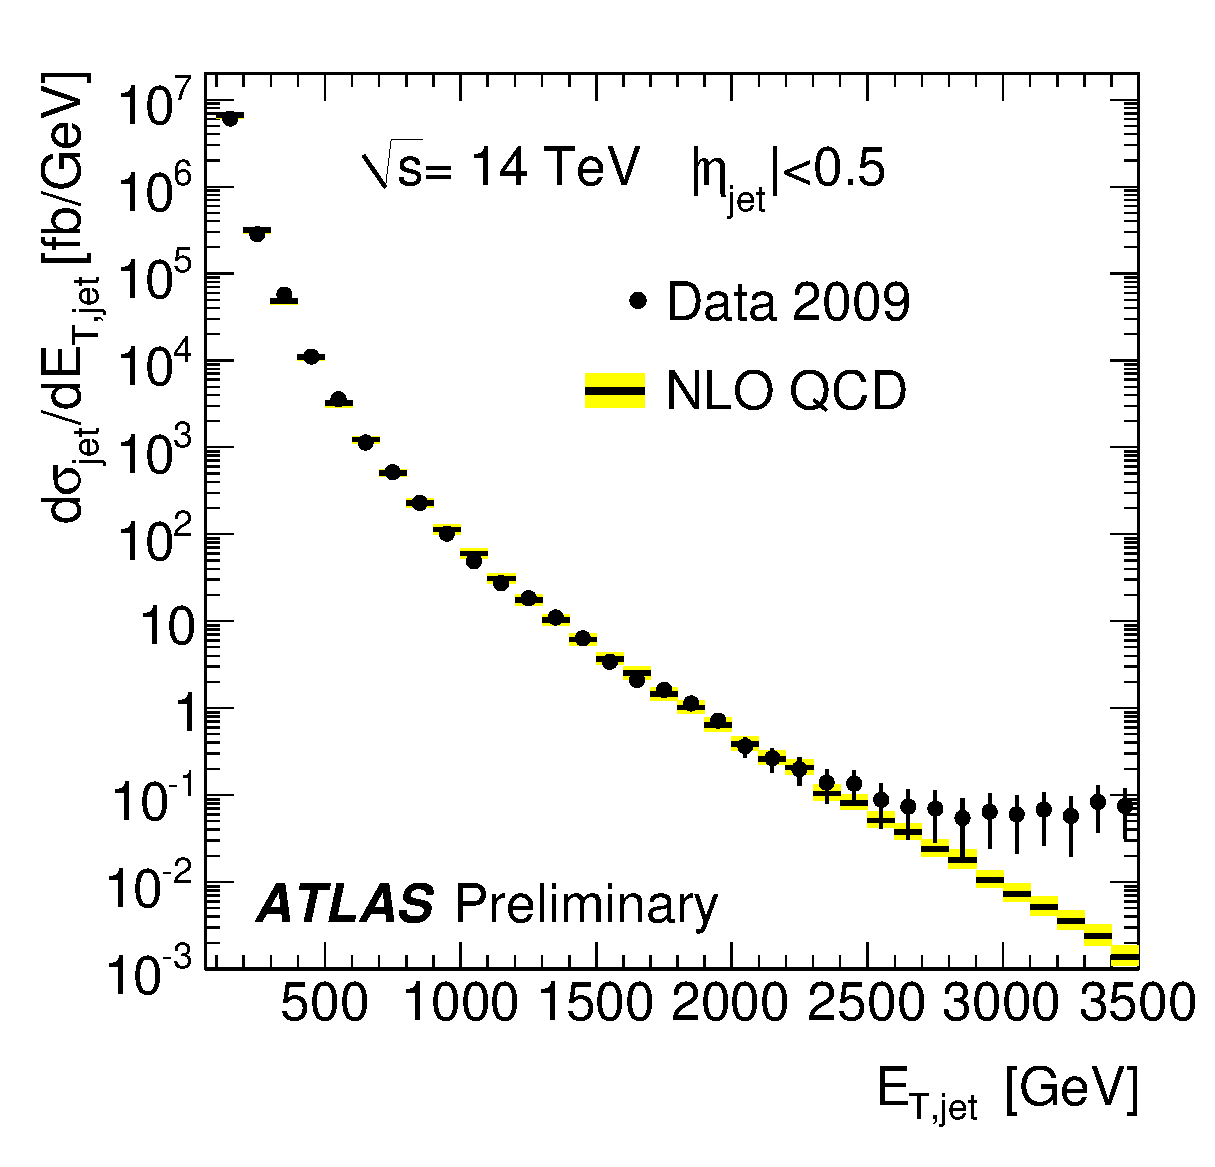
\includegraphics[width=0.5\columnwidth]{AtlasExample}
  \caption{An example ATLAS figure.}
  \label{fig:example}
\end{figure}

A figure with subfigures can be made as shown in the example of
Figure~\ref{fig:subfigexample}. In this example the \Package{subfig} package is used.
The syntax with the \Package{subcaption} and \Package{subfigure} packages is very similar.
The following commands were used to produce Figure~\ref{fig:subfigexample}:
{\footnotesize
\begin{verbatim}
\begin{figure}[htbp]
  \centering
  \subfloat[One subfigure example]{
    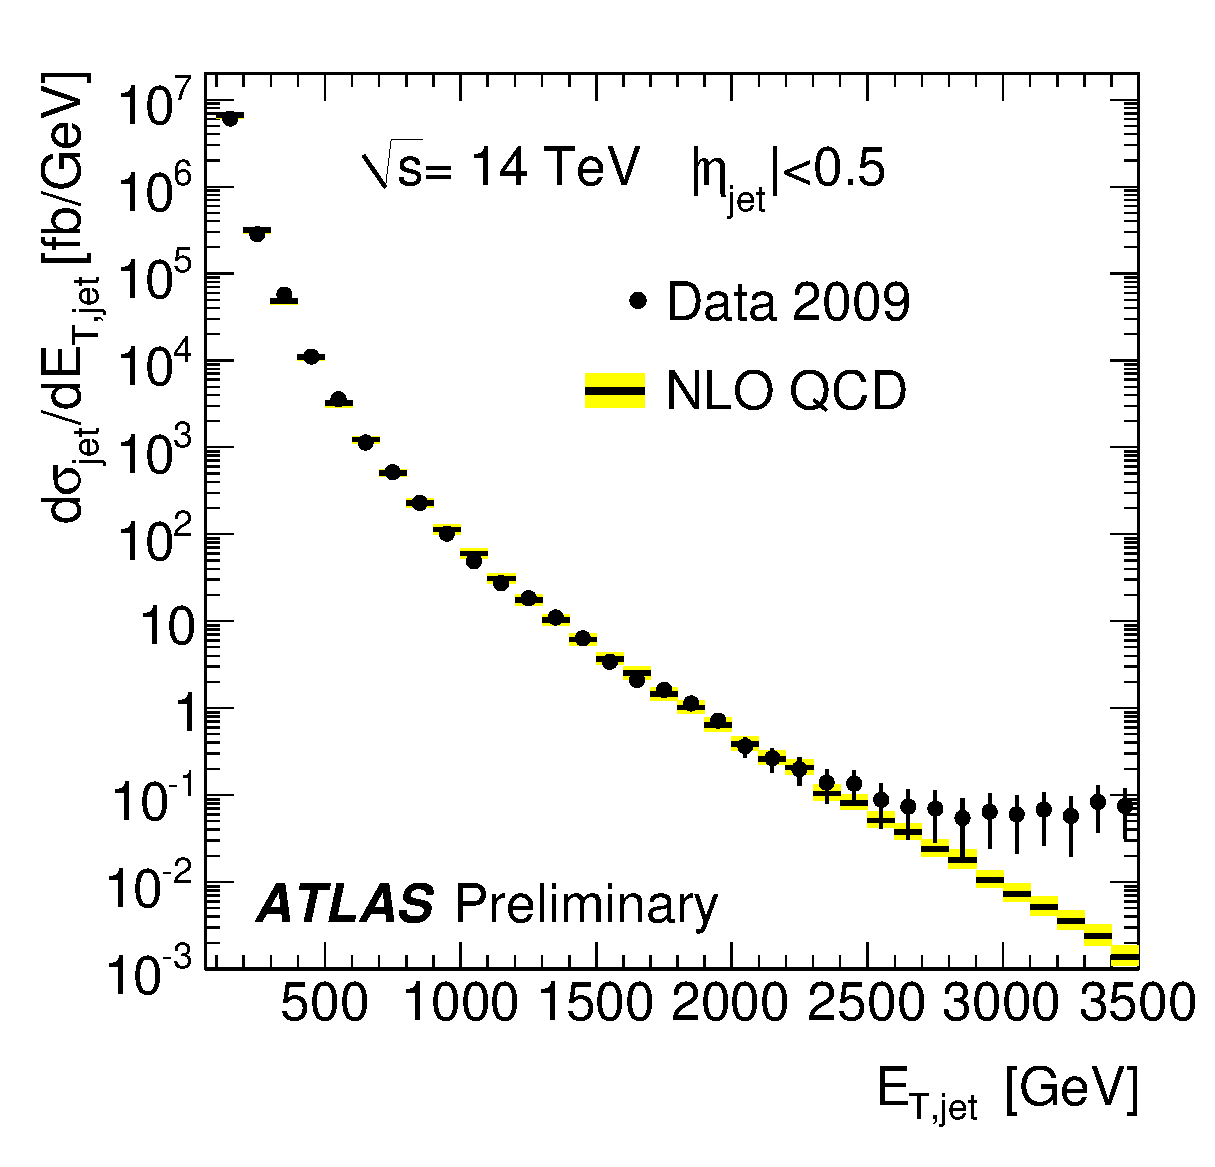
\includegraphics[width=0.45\textwidth]{AtlasExample}
    \label{fig:SubfigureExample1}
  }
  \subfloat[Another subfigure example]{
    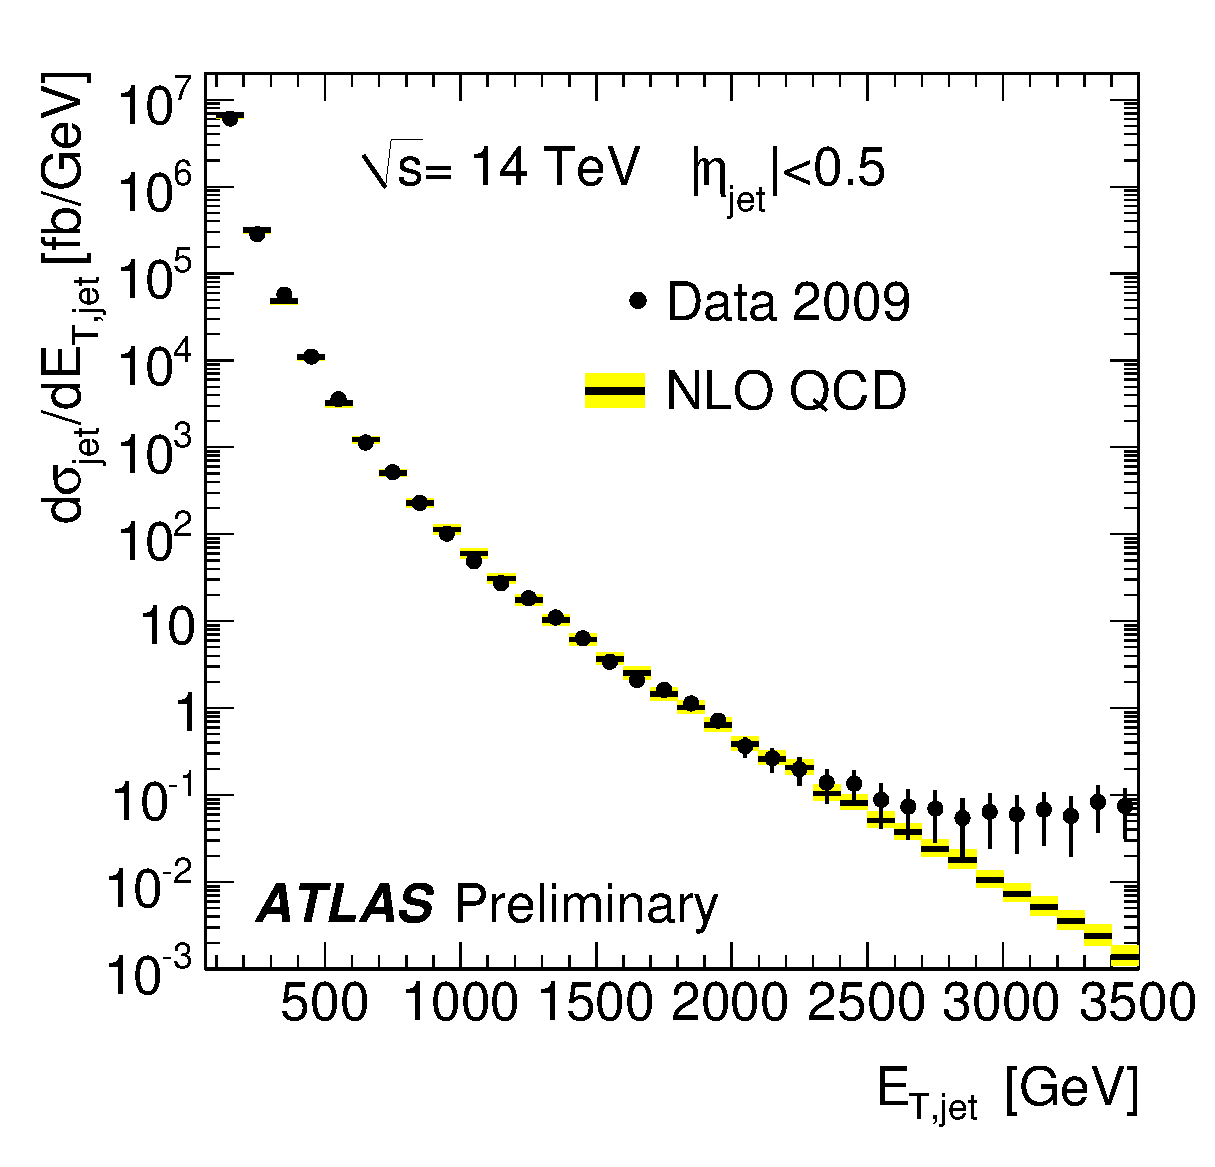
\includegraphics[width= 0.45\textwidth]{AtlasExample}
    \label{fig:SubfigureExample2}
  }
  \caption{Subfigure example.
    \protect\subref{fig:SubfigureExample1} shows the cross-section as a function of $E_{\text{T,jet}}$ and 
    \protect\subref{fig:SubfigureExample2} shows exactly the same thing!}
  \label{fig:subfigexample}
\end{figure}
\end{verbatim}
}

You refer to the main figure using the usual \verb|\ref| command, e.g.\ see \Fig{\ref{fig:subfigexample}}.
You can refer to the subfigures using either the syntax \verb|\ref{fig:subfiglabel}| 
(e.g.\ see \Fig{\ref{fig:SubfigureExample2}}) or\\
\verb|\ref{fig:mainfiglabel}\subref{fig:subfiglabel}|
(e.g.\ see \Fig{\ref{fig:subfigexample}\subref{fig:SubfigureExample1}}).
Note that if you use the \Package{subfig} package and want to use the labels of the subfigures in the caption,
you have to use the syntax \verb|\protect\subref{fig:SubfigureExample1}|.
The packages \Package{subfigure} and \Package{subcaption} do not need protect, but it does not do any harm.

\begin{figure}[htbp]
  \centering
  \subfloat[One subfigure example.]{
    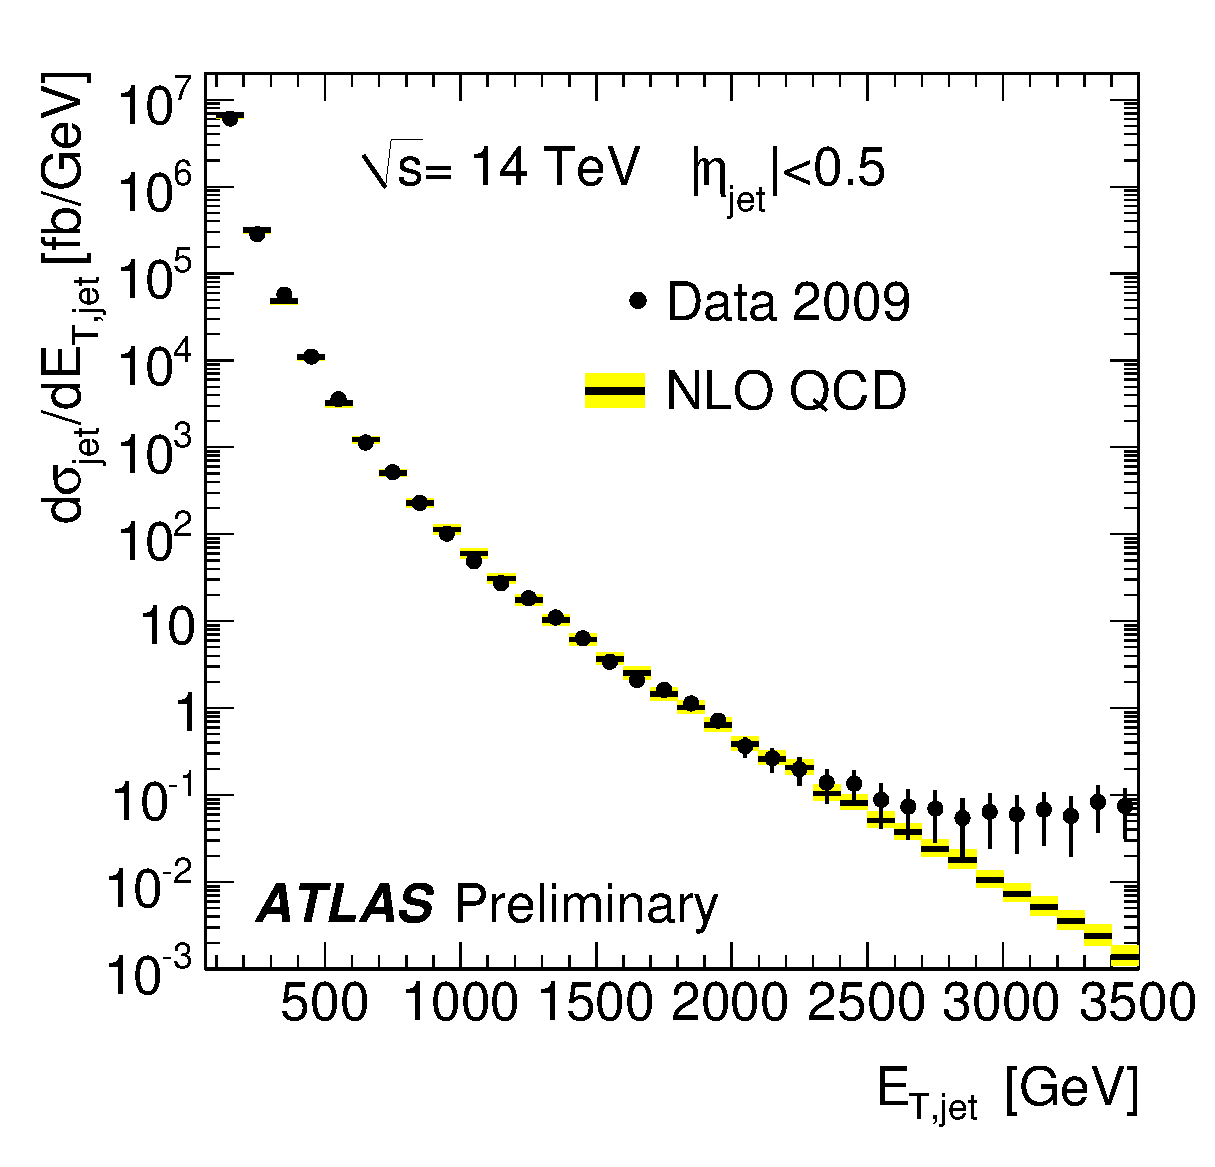
\includegraphics[width=0.45\textwidth]{AtlasExample}
    \label{fig:SubfigureExample1}
  }
  \subfloat[Another subfigure example.]{
    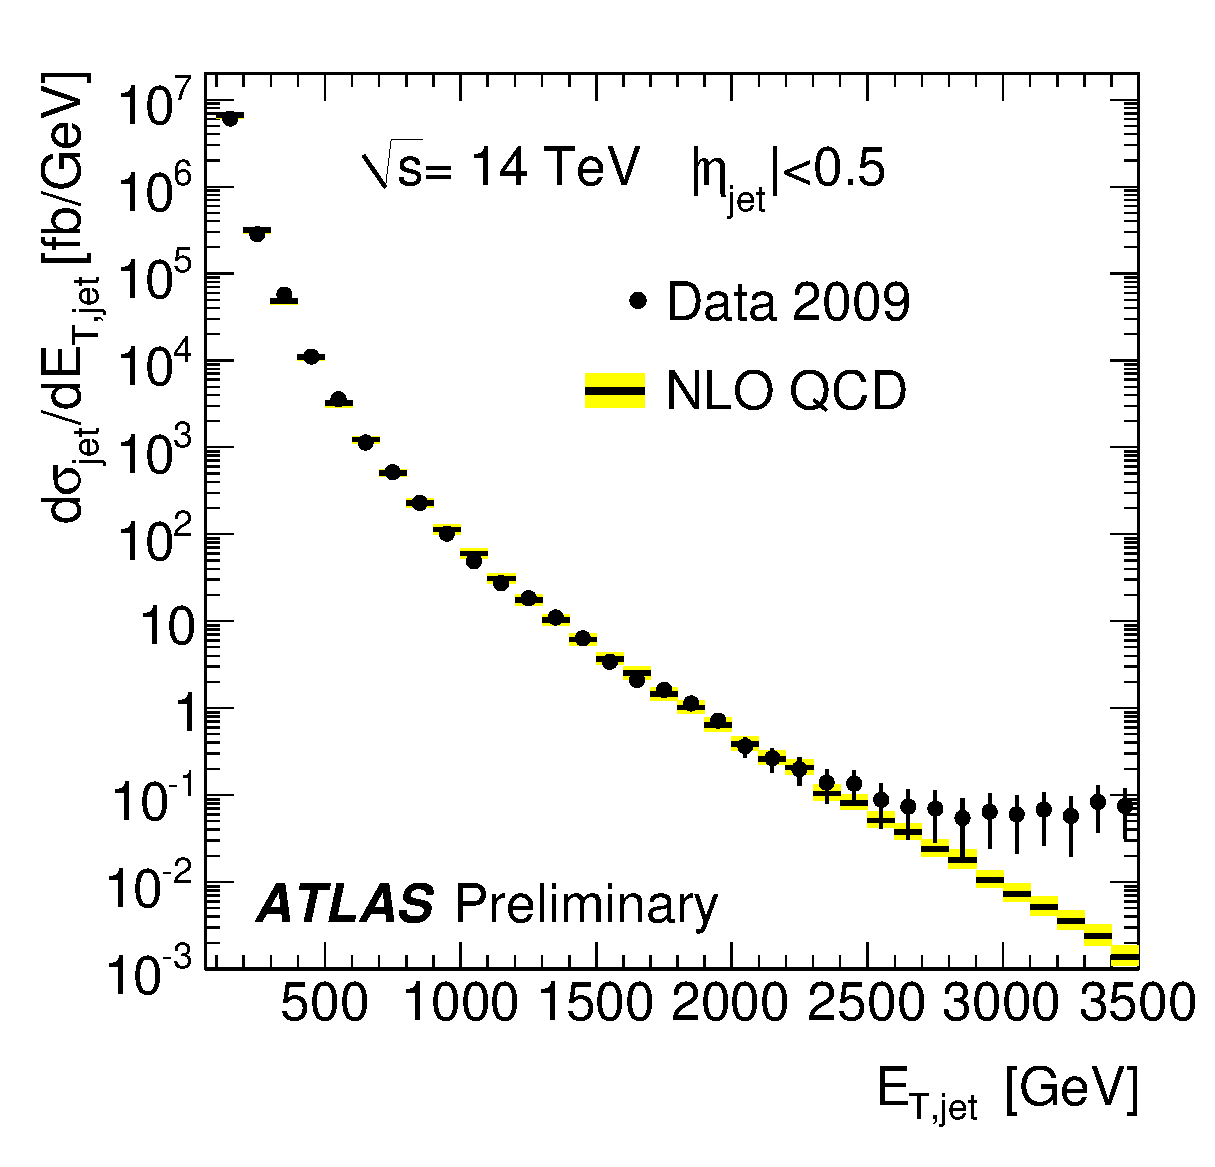
\includegraphics[width= 0.45\textwidth]{AtlasExample}
    \label{fig:SubfigureExample2}
  }
  \caption{Subfigure example.
    \protect\subref{fig:SubfigureExample1} shows the cross-section as a function of $E_{\text{T,jet}}$ and 
    \protect\subref{fig:SubfigureExample2} shows exactly the same thing!}
  \label{fig:subfigexample}
\end{figure}


%-------------------------------------------------------------------------------
\subsection{Positions of figures and tables}

In an ATLAS paper, all figures and tables should be printed before the conclusions.
You can achieve this by using the macro \Macro{FloatBarrier} from the
\Package{placeins} package.

In general, as mentioned above, you should separate the figure and table environments from the text by blank lines.
This helps the line numbers. The standard options to use for the placement are \Option{[htbp]}.


%-------------------------------------------------------------------------------
\subsection{Math mode macros}%
\label{sec:math}
%-------------------------------------------------------------------------------

The correct \LaTeX\ macros for math mode are \textbackslash(\ldots\textbackslash)
and not \(\$\ldots\$\) (which are \TeX\ primitives),
even though the \TeX\ primitives are used by most people.
\ADOCnew{06-00-00} The standard ATLAS bibliography and template files use the correct \LaTeX\ macros and
the documentation, example files will also be adjusted to use them.

If you are using a version of \LaTeX\ from before 2015, you may have problems
if you use the \LaTeX\ delimiters in captions and want to make as list of tables or figures.
If this is the case, just switch to \TeX\ primitives in the caption (or subcaption).


%-------------------------------------------------------------------------------
\subsection{\pT or \ET, that is the question}

Bold math should be automatically invoked in titles.
This short section tests whether that works properly.
It is of course good if things like \pT and \ET are automatically in bold face in
a header and normal font in the text (and table of contents).

With the current setup, this works OK. 
However, if you just use the option \Option{koma}, which then typesets titles using a sans serif font,
the $p$ and $E$ are typeset with a serif font and \textsf{T} is typeset with a sans serif font,
which is probably not what one wants!
Work is still ongoing to find the optimal set of options
--- search for \texttt{detect} in the \Package{siunitx} manual, to see the complete set of possibilities.
This is not a problem for the ATLAS preprint style as it uses a serif font for the section titles.


%------------------------------------------------------------------------------
\section{Recommended packages}

A vast number of \LaTeX\ packages are available.
In this section I collect a few useful packages that I recommend using.

\begin{description}
  \item[cleveref] Means that constructs like \verb|Fig.~\ref{fig:one}| or
  \verb|\Fig{\ref{fig:one}}| are no longer necessary.
  Instead just use \verb|\cref{fig:one}|.
  The package decides if it is a figure, table or equation and
  adds the appropriate text.
  At the beginning of sentences use \Macro{Cref}.
  This package is included by default if you use \Package{atlaspackage}.
  You can customise its use with the \Option{capsref} and \Option{abbrevref} options.
  If you include the package yourself, use \Macro{usepackage\{cleveref\}} to get \enquote{fig.} etc. and
  use \Macro{usepackage[capitalize]\{cleveref\}} to get \enquote{Fig.} etc.

  \item[heppennames] A package that defines most elementary particle, mesons and baryons in a
  consistent way. Optionally the symbols can be upright or italic.
  The package is included if you pass the option \Option{hepparticle} to \Package{atlasphysics}.
  You can use the package \Package{hepnicenames} instead, which uses more intuitive names for the particles,
  but is not as systematic.

  \item[diffcoeff] A useful package for differentials.
  \ADOCnew{14.0.0} The package is no longer included if you pass the option \Option{full} to \Package{atlaspackage},
  as its syntax has changed too often in the past years.
  If you pass the option \Option{diffcoeffISO=false}
  a slanted \textit{d} is used in differentials,
  while an upright \textrm{d} is used for other languages.
  % diffcoeff tweaks for other TeX Live versions.
  % Have to change things for 2023 (version 5) version of diffcoeff.
  % \ifthenelse{\AtlasTeXLiveVersion < 2018}{%
  In version 5 (released in 2023), the \Macro{dl} command includes a small space before the differential,
  while there is no space on older versions.
  For ATLAS papers you should use the older version syntax, as arXiv uses an older version of \Package{diffcoeff}.
  For this reason, the package is included in \Package{atlaspackage} using the command
  \Macro{RequirePackage\{diffcoeff\}[=v4]}.
  Hence, one should use a syntax like \Macro{dl2\{x\}},
  e.g.\ \verb|\int f(x) \dl2{x}| gives
  \ifthenelse{\AtlasTweakYear > 2017}{\(\int f(x) \dl2{x}\)}{XXX},
  while \verb|\int f(x) \dl0{x}| or \verb|\int f(x) \dl{x}| gives  
  \ifthenelse{\AtlasTweakYear > 2017}{\(\int f(x) \dl0{x}\).}{XXX.\\
    \emph{Examples are not complete as some \Package{diffcoeff} package options are not available for older versions of TeX Live.}
  }
  
  Alternatives are \Package{esdiff} and \Package{derivative},
  but the \Package{derivative} is probably too new to be used in papers.
  You can use a package such as \Package{braket} for Dirac notation etc.

  The package \Package{physics} can also be used for differentials, matrices and more.
  As the name suggests it is geared to physics usage.
  However, the \LaTeX\ community is not very enthusiastic about the way the package is written.
  
  The \Package{commath} package is another alternative,
  but I find the \Package{physics} package to be more reliable when different fonts are used.

  \item[todonotes] Very nice package for adding notes.
  It is used by the \File{atlastodo.sty} style file.
  See \File{atlascomment.sty} for a further example.
\end{description}


%------------------------------------------------------------------------------
\subsection{Other (useful) packages}

In this section I collect a few useful packages that may be useful when preparing a document.
Note that I have only had a cursory read of their documentation,
so some work amy be needed to get them working as they are supposed to.
\begin{description}
  \item[snapshot] As the first paragraph of the documentation quotes:
    \begin{quotation}
      The \Package{snapshot} package helps the owner of a \LaTeX\ document obtain a list of the external dependencies of the document,
      in a form that can be embedded at the top of the document.
      To put it another way, it provides a snapshot of the current processing context of the document,
      insofar as it can be determined from inside \LaTeX.
  \end{quotation}
  It can also be used to arrange that the document is processed with the same versions of everything.
  I tried the package once, and it gave an error compiling.
  However, even if the compilation gives and error
  you can look at the resulting \File{.dep} file to get a list of all packages and versions used in a document.
  This may be helpful for debugging problems.

  \item[changes] The \Package{changes} package is another way of recording changes and adding comments.
    The \Package{todonotes} package is used to do some of this and is integrated into the \Package{atlastodo} style file.
    The \Package{changes} is supposed to work much like change markup in LibreOffice, Microsoft Office etc.
\end{description}


%-------------------------------------------------------------------------------
\section{Remarks on units and symbols}%
\label{sec:siunitx}
%-------------------------------------------------------------------------------

It is highly recommended to use a units package to format your units properly.
The package \Package{siunitx} works very well and is the package of choice.
Alternatives include \Package{units} and \Package{hepunits},
which is based on \Package{SIunits}.

The basic command to use in \Package{siunitx} is \verb|\qty{20}{\GeV}| to get
\qty{20}{\GeV}. 
There are also several other useful commands for specifying ranges:
\verb|\numrange| for a range of numbers and \verb|SIrange| for a range of numbers with a unit. 
Options exist for specifying how they are formatted.
The options can be set for an individual command or for the whole document.
For example, in this document I have specified the options:\\
\verb|\sisetup{separate-uncertainty, range-units=single, list=units=single}|
and\\
\verb|\sisetup{group-digits=integer, group-minimum-digits=4, detect-all}|.

In addition several extra units are defined:
\begin{itemize}
\item \verb|\micron| for \unit{\micron};
\item \verb|\mrad| for \unit{\mrad};
\item \verb|\nb| for \unit{\nb};
\item \verb|\pb| for \unit{\pb};
\item \verb|\fb| for \unit{\fb}.
\end{itemize}
Use the syntax \verb|\qty{20.3}{\per\fb}| to get \qty{20.3}{\per\fb}.

Some things to note about using \Package{siunitx}:
\begin{itemize}
\item It tries to isolate itself from other packages.
  If you just want to write \unit{\GeV} in your text,
  then you must write \verb|\unit{\GeV}|.
\item It also contains two new column specifiers for tables ``S'' and ``s'',
  which are extremely useful for formatting tables properly.
\end{itemize}

% The option names are somewhat different for \TeX\ Live 2009,
% as this contained \Package{siunitx} Version 1.
% You can use the older options by including \Package{atlaspackage} with the 
% option \Option{texlive=2009}.
% You also have to turn off the inclusion of \File{atlasunits.sty} by including the option \Option{units=false} with
% the \Package{atlasphysics} package.


%-------------------------------------------------------------------------------
\section{\texttt{atlaslatex} directories and Git}
\label{sec:gitsvn}
%-------------------------------------------------------------------------------

There is some flexibility in how you set up your directory structure for using \Package{atlaslatex}.
By default the \Package{atlaslatex} style files are in the \File{latex} subdirectory and the
logos are in \File{logos}. This structure assumes that you will make a separate directory tree
for each document that you create.
If you want to include these files in Git or SVN, note that you only need to add the
\File{latex}, \File{logos} and \File{bib} directories of the \Package{atlaslatex} package to Git.
In order to create a new document, you also need the \File{template} directory.
For a paper, you also need the \File{acknowledgements} directory.

If you want use a centrally installed \Package{atlaslatex} package, then you would usually unpack the\\
\File{atlaslatex-X.Y.Z.tds.zip} file into your \File{texmf} tree --- see \cref{sec:texmf}.

If you want to use another setup, you should adjust the directory in \File{latex/atlaslatexpath.sty} appropriately.
This would enable you to maintain a single copy of each \Package{atlaslatex} version and easily switch between versions.
For example, you specify:
\verb|\def\input@path{{../atlaslatex-10.0.0/latex/}}|
in \File{latex/atlaslatexpath.sty}
to use version 10.0.0 of the \Package{atlaslatex} package, which you have unpacked into the directory tree
\File{../atlaslatex-10.0.0}.
Such a structure makes it very easy to switch between \Package{atlaslatex} versions without breaking anything!

% If you want to use another setup, you should set the variable \Macro{ATLASLATEXPATH} appropriately
% at the beginning of your document. This would enable you to maintain a single copy of each 
% \Package{atlaslatex} version and easily switch between versions.
% For example, you give the command\\
% \verb|\newcommand*{\ATLASLATEXPATH}{../atlaslatex-01-08-00/}|
% to use version 01-08-00 of the \Package{atlaslatex} package, which you have unpacked into the directory tree
% \File{../atlaslatex-01-08-00}.
% Such a structure makes it very easy to switch between \Package{atlaslatex} versions without breaking anything!


%-------------------------------------------------------------------------------
\section{Platforms and \LaTeX\ versions}
\label{sec:version}
%-------------------------------------------------------------------------------

The \Package{atlasdoc} class should in principle work both with \LaTeX{} and pdf\LaTeX{}.
However, the collection is no longer tested with \LaTeX,
so I strongly recommend to use pdf\LaTeX, which is the default.

I would expect everything to work with \TeX\ Live 2013 or later.
% You should just set the option \Option{texlive} appropriately.
% This is best done in the document class, as the option is then passed to all other packages.
Examples of changes include some option names for \Package{siunitx}.

% If for example you have \TeX\ Live 2013, add the option \Option{texlive=2013} to the document class.
% This will then include \Package{siunitx} with the correct options for Version 1.
% It will also switch to \Option{unit=false} to \Package{atlasphysics}
% and use option \Option{txfonts} in \Package{atlasdoc}.

\ADOCnew{04-00-00} If you use the \Package{biblatex} package,
the default is to use the \texttt{biber} backend.
% For \TeX\ Live versions earlier than 2013, it may be better to use \texttt{bibtex}.
% To do this, pass the option \Option{backend=bibtex} to \Package{atlaspackage}.

The \Package{atlaslatex} package should work under Linux, macOS and Windows.
Details on the installations that I use for testing things
and how you should set up your system can be found on the PubCom LaTEX FAQ~\cite{latex-faq}.


%-------------------------------------------------------------------------------
\section{Installation of \Package{atlaslatex} in \File{texmf} tree}%
\label{sec:texmf}
%-------------------------------------------------------------------------------

As discussed above, the \texttt{atlasdoc} class and the style files can all be found in the 
\File{latex} subdirectory. The template documents are usually set up to pick up the style files from there.
If you want to use the centrally installed version,
you should first copy \File{Makefile}, the \File{template} directory and the \File{bib} directory from 
\File{\$\{HOME\}/texmf/source/atlaslatex} to the directory where you want to create your document.
For the main document, you can then use the command 
\texttt{make newpapertexmf}, \texttt{make newnotetexmf} or \texttt{make newbooktemmf} to get a template which uses the
centrally installed style files.

If you want to install the package in a central area, use the \File{atlaslatex-X.Y.Z.tds.zip} file.
Change your directory to \File{\$\{HOME\}/texmf} and unzip the file there.
% To do it by hand you can do:
% \begin{itemize}
% \item unpack the tarball;
% \item copy the \texttt{latex} directory to \File{\$\{HOME\}/texmf/tex/latex/atlaslatex};
% \item copy the contents of the \File{bib} directories 
%   to \texttt{\$\{HOME\}/texmf/bib}.
% \end{itemize}
% It is more complicated to checkout part of a Git repository.
% Hence the method described above is the recommended way of installing
% \Package{atlaslatex} in your \File{texmf} tree.
% You can also checkout the two directory trees from SVN:
% {\small
% \begin{verbatim}
% cd ~/texmf/tex/latex
% svn co svn+ssh://svn.cern.ch/reps/atlasgroups/pubcom/latex/atlaslatex/trunk/latex atlaslatex
% cd ~/texmf
% svn co svn+ssh://svn.cern.ch/reps/atlasgroups/pubcom/latex/atlaslatex/trunk/bibtex
% \end{verbatim}
% }
% The advantage of using SVN is that you can keep the package up to date, by just giving the command
% \verb|svn update| in the two directories.
% If you already have a \File{bibtex} directory,
% first move it out of the way, then checkout from SVN
% and then move the contents of the old directory back into the \File{bibtex} tree.

% Under Windows, it appears to be better to use \texttt{https} instead of \texttt{svn+ssh}.
% You should therefore checkout:\\
% \verb|https://svn.cern.ch/reps/atlasgroups/pubcom/latex/atlaslatex/trunk|

In the template files, you have to use the command
\texttt{make newpapertexmf} or \texttt{make newnotetexmf} or simply comment out the line
\verb|\RequirePackage{latex/atlaslatexpath}|
% \begin{center}
%   \begin{tabular}{ll}
%     From & To \\
%     \midrule
%     \verb|\newcommand*{\ATLASLATEXPATH}{latex/}|    & \verb|\newcommand*{\ATLASLATEXPATH}{}| \\
%   \end{tabular}
% \end{center}

If you are using traditional \BibTeX\ you also have to change\\
\verb|\bibliographystyle{bib/bst/atlasBibStyleWoTitle}| to\\
\verb|\bibliographystyle{atlasBibStyleWoTitle}|

The \Option{texmf} option in \Package{atlasphysics} is not strictly necessary if you use the class \Package{atlasdoc},
but it does not do any harm.


\appendix
\clearpage
%-------------------------------------------------------------------------------
\section{Makefile}
%-------------------------------------------------------------------------------
\label{sec:makefile}

This section documents what the \File{Makefile} does when it creates a new document
or compiles one.

When a new paper draft is created using the command\\
\texttt{make newpaper BASENAME=GROUP-YYYY-XX-PAPER}\\
the following files are created in the main directory.
If a template filename is given in the table
it is taken from the \texttt{template} directory,
otherwise empty files are created.
\begin{center}
  \begin{tabular}{ll}
    \mcc{\texttt{template}} & \mcc{\texttt{main}} \\
    \midrule
    \texttt{atlas-paper.tex} & \texttt{GROUP-YYYY-XX-PAPER.tex} \\
    \texttt{atlas-paper-metadata.tex} & \texttt{GROUP-YYYY-XX-PAPER-metadata.tex} \\
    \texttt{atlas-auxmat.tex} & \texttt{GROUP-YYYY-XX-PAPER-auxmat.tex} \\
    \texttt{atlas-hepdata.tex} & \texttt{GROUP-YYYY-XX-PAPER-hepdata.tex} \\
    & \texttt{GROUP-YYYY-XX-PAPER-defs.sty} \\
    & \texttt{GROUP-YYYY-XX-PAPER.bib}
  \end{tabular}
\end{center}
The following string substitutions are made in \texttt{GROUP-YYYY-XX-PAPER.tex}:
\begin{center}
  \begin{tabular}{ll}
    \mcc{Old string} & \mcc{New string} \\
    \midrule
    \texttt{atlas-document} & \texttt{GROUP-YYYY-XX-PAPER}
    % \texttt{texlive=2020} & \texttt{texlive=YYYY} \\
  \end{tabular}
\end{center}
The \TeX\ Live version is changed to \texttt{YYYY} (if given). Otherwise it is set to 2020.

The same thing is done for an ATLAS supporting note made with the command\\
\texttt{make newnote BASENAME=GROUP-YYYY-XX-INT1},\\
except that the main file template is taken from
\texttt{atlas-note.tex},
the metadata template is taken from \texttt{atlas-note-metadata.tex},
and the auxiliary material and HEPData files are not created.

The standard sequence of commands to compile a document is
\texttt{pdflatex, biber, pdflatex, pdflatex}.
You can change the \texttt{\%.pdf} target if necessary.
Better is to use \texttt{latexmk} via the target \texttt{run\_latexmk}.
I recommend you set this as the default command.

%-------------------------------------------------------------------------------
\section{Journal templates}
%-------------------------------------------------------------------------------
\label{sec:journal}

This section contains some information on where the \LaTeX\ templates for the different journals can be found and how to use them.
With the advent of the ATLAS preprint style and its use for ATLAS publications, 
it should no longer be necessary to format papers in the style used by the journals.
However, for papers that are written by a limited number of authors
the journal may require that the paper be submitted using its style.

The directory \File{journal} contains a very basic paper outline with the preamble needed for different journals.
So far the \Package{atlaslatex} package has been tested with the classes for Elsevier and APS journals and the style file used for JHEP and JINST.
The journal templates turn off the use of \Package{biblatex}
by adding the option \Option{biblatex=false} to \Package{atlaspackage}.
I have not tested if it is possible to use \Package{biblatex}.

\begin{description}
\item[Elsevier]Elsevier uses the \texttt{elsarticle} class which should be already installed if you have a standard 
  \TeX\ Live distribution. 
  It can also be found at \url{http://www.elsevier.com/locate/latex}.
  
\item[APS]APS journals use REV\TeX. This is also usually installed.
  It can also be found at \url{https://journals.aps.org/revtex}.
  Note that you have to specify the author after \verb|\begin{document}| with this class.
  Hence you should comment out the definition in your metadata file,\\
  e.g.\ \File{mydocument-metadata.tex}.
  If you want line numbers in a document typeset using REV\TeX, it is best to use the class option \Option{linenumbers}.
  In addition you should include \Package{atlaspackage} with the option \Option{lineno=false}.
  
\item[JHEP]The package can be downloaded from \url{http://jhep.sissa.it/jhep/help/JHEP_TeXclass.jsp}.
  It contains a style file \File{jheppub.sty} as well as a \BibTeX\ style file \File{JHEP.bst}. 
  If the author of the paper is not the the ATLAS Collaboration,
  you should use the macros \Macro{author} and \Macro{affiliation} to specify the names and their instiutions (see the documentation)
  and should NOT include the \Package{authblk} package.

\item[JINST]The package can be downloaded from \url{https://jinst.sissa.it/jinst/help/helpLoader.jsp?pgType=author}.
  It contains a style file \File{jinstpub.sty} as well as a \BibTeX\ style file \File{JHEP.bst}.
  The information on authors is the same as for JHEP.
\end{description}


%-------------------------------------------------------------------------------
\section{From \texttt{atlasnote} to \texttt{atlasdoc}}
\label{sec:oldnote}
%-------------------------------------------------------------------------------

The \texttt{atlasdoc} class replaces and supersedes \texttt{atlasnote}.
The decision was taken to give the class a new name, as it is supposed to be
able to be used for (almost) all ATLAS documents.
Some small changes in the user setup are necessary to use the new
class, style files and templates.

All style files are collected in the \texttt{latex} subdirectory.
It is assumed that this directory is a direct subdirectory of you main \LaTeX\ file.
If you want to keep the style files in a central place you can either put them in
\verb|${HOME}/texmf/tex/latex| or create a link from your main directory to the location of
your \texttt{latex} directory.

The main changes the user has to make are:
\begin{itemize}
\item Change the class name from \texttt{atlasnote} to \texttt{latex/atlasdoc};
\item Specify the document language as an option: UKenglish or USenglish;
\item Add \verb|\usepackage{latex/atlaspackage}| at the beginning of the document;
\item Change \verb|\usepackage{atlasphysics}| to \verb|\usepackage{latex/atlasphysics}|; 
\item Use the macro \Macro{AtlasTitle} instead of \Macro{title}.
\end{itemize}

The language specification means that dates etc.\ are also formatted according to 
the document language. 
If you use the package \Macro{csquotes}, quotation symbols are also consistently and properly set
when you use \Macro{enquote}.

All the documentation uses \texttt{biblatex} and \texttt{biber} instead of traditional \BibTeX.
The templates provide information on how to make the change in your own document.
The default document settings also use \texttt{biblatex} and \texttt{biber}.

\ADOCnew{01-00-00} The same macro names are used in both \Package{atlasdoc} and
\Package{atlascover} so that title, journal, version number and abstract only need to be specified once.
This means that if you start from an old preamble the following changes should be made:
\begin{center}
  \begin{tabular}{ll}
    Old	& New\\
    \midrule
    \Macro{title} & \Macro{AtlasTitle}\\
    \Macro{draftversion} & \Macro{AtlasVersion}\\
    \Macro{atlasnote} & \Macro{AtlasNote}\\
    \Macro{journal} & \Macro{AtlasJournal}\\
    \Macro{abstracttext} & \Macro{AtlasAbstract}
  \end{tabular}
\end{center}
If you use the old macro names 
\Macro{draftversion}, \Macro{journal}, \Macro{abstracttext},
they will continue to work in the document itself, but not on the cover page.

When you want to circulate a draft with cover pages, 
you also need to set the macro \Macro{AtlasRefCode}.
This replaces \Macro{AtlasCoverNumber} as it is used in several places.

The class and style files have been cleaned up and things 
that were thought to no longer be necessary have been removed.
% These pieces have been collected in \texttt{obsolete/atlasnote-obsolete.sty} in case they are needed.
% If something important has got lost, please let me know.

The \Package{subfigure} package has been replaced with \Package{subfig}, as \Package{subfigure} is now deprecated.
If you use \Package{subfig}, then you have to use \Macro{subfloat} instead of \Macro{subfigure}.
If you want to continue to use \Package{subfigure} include \Package{atlaspackage} with the option
\Option{subfigure=true}. 
You should also comment out the \Macro{usepackage\{subfigure\}}.

Similarly, if you do not want to include \Package{siunitx} set
the option \Option{siunitx=false}.

The option \verb|\skipbeforetitle{<length>}| used to set the distance between
the title page header and the note title. 
Given that stretchable space is now used, such an option is no longer appropriate.
It can be given, but will be ignored.
%The default value should be fine for most notes, but in case you have a long list of
%authors or a lengthy abstract you can use this command to buy
%some extra space. Note that \verb|<length>| can also be negative
%(use it at your own risk!).

%-------------------------------------------------------------------------------
\section{History}
%-------------------------------------------------------------------------------

Quite a lot of people have contributed to the ATLAS \LaTeX\ templates over time.
Marco Delmastro set them up in the first place and added a number of improvements over time.
Mike Vetterli implemented several changes to the cover pages, including switching to two pages.
Cristina Oropeza, Vasia Mitsou, Chris Hays and Mike Vetterli all made contributions to the preprint cover page.

Sven Menke provided the code so that bold math works in titles correctly.
Thorsten Kuhl had the idea of defining \Macro{ATLASLATEXPATH}, which makes things much more flexible.
Some problems occurred with this scheme \TeX{} Live 2020.
As a result the use of \Macro{ATLASLATEXPATH} was replaced with the \File{atlaslatexpath.sty} style file.

Juan Pedro Araque has done most of the work setting up the PO-GitLab project.
This resulted in a much smoother submission process for papers and
an improved handling of auxiliary material.

Knut Zoch provided the code that fixed the line numbering problems with AMS Math \LaTeX\ environments.


%-------------------------------------------------------------------------------
\subsection{Changes in \texttt{atlaslatex-14.0.0}}
\label{sec:atlaslatex14}
%-------------------------------------------------------------------------------

\ADOCnew{14.0.0} no longer needs or uses the \Option{texlive} option,
which used to be passed to the document class.

Internally \Macro{@ifpackaglater} and \Macro{@ifclasslater} are now used instead.
Some of the documentation and test files do need such a variable,
but this is now set only in those documents where it is needed.

Th package \Package{diffcoeff} is no longer included when the \Option{full}
is passed to \Package{atlaspackage}, as its syntax and options have changed too often.


%-------------------------------------------------------------------------------
\subsection{Changes in \texttt{atlaslatex-10.0.0}}
\label{sec:atlaslatex10}
%-------------------------------------------------------------------------------

\ADOCnew{10.0.0} switches to Semantic Versioning.

The major change in this version is in the way that the class and style files are included.
This had to be changed as the result of a bug introduced in the October 2020 update of \LaTeX.
The \LaTeX{} update led to options being ignored when passed to a document class or a style file,
if the filename contained a directory.
While this bug will probably be fixed at some point,
it in general appears to be better to adjust the macro \Macro{input@path}
to specify the directory that should be searched for the ATLAS \LaTeX{} packages.
Hence a new style file \File{atlaslatexpath.sty} has been introduced and should be loaded using
\begin{tcblisting}{listing only}
\RequirePackage{latex/atlaslatexpath}
\end{tcblisting}
before the \Macro{documentclass}.

This change implies that all main files have to be updated.
A script \File{scripts/atlaslatex\_2020.sh} is provided that should make the necessary changes.


%-------------------------------------------------------------------------------
\subsection{Changes in \texttt{atlaslatex-05-00-00}}
\label{sec:atlaslatex5}
%-------------------------------------------------------------------------------

\ADOCnew{05-00-00} is the first version set up
to be fully compatible with the PO-GitLab scheme for papers.

Separate (dummy) files for auxiliary material and HEPData tables are created for new papers.
The \verb|make auxmat| command has been renamed to \verb|make newdata|,
as the auxiliary material for the webpage is now separated
from a separate file for tables etc.\ for HEPData.


%-------------------------------------------------------------------------------
\subsection{Changes in \texttt{atlaslatex-04-00-00}}
\label{sec:atlaslatex4}
%-------------------------------------------------------------------------------

\ADOCnew{04-00-00} The \File{Makefile} for \Package{atlaslatex}
has been restructured to reduce duplications and make separate commands for a new paper and a new note.
\texttt{biber} is now the default backend for \Package{biblatex},
as this allows the use of the \enquote{related} field for Errata.
Errata are included in the ATLAS bibliography file.
Metadata for notes and papers are now separate templates to prepare for them being created directly from Glance.
This is the first version that is designed for the Glance/Git integration.
As the above changes are quite major, there is a jump in the main version number.


%-------------------------------------------------------------------------------
\subsection{Changes in \texttt{atlaslatex-02-00-00}}
\label{sec:atlaslatex2}
%-------------------------------------------------------------------------------

\ADOCnew{02-00-00} Only the \KOMAScript\ classes are supported.
At the same time, the option BOOK was introduced, which uses \Package{scrbook} as the base class.
This is more suitable for long documents such as a TDR.

Several options, which make maintenance more difficult have been removed:
\Option{maketitle}, \Option{nomaketitle}, \Option{koma}.
In addition, support for \TeX\ Live versions older than 2009 has been removed.
% A version of the class with these options, which should still work with \TeX\ Live 2007,
% but without the \Option{BOOK} option is available as \File{atlasdoc1.cls}.
% However, the class (\Package{atlasdoc1}) will not be actively maintained or developed any more.
% If you want to explicitly load the \Package{atlascover} package,
% you should load \Package{atlascover1} when using \Package{atlasdoc1}.

The options \Option{cernpreprint}, \Option{preprint} and \Option{auxmat} are no longer available
in \Package{atlascover}.
You should pass these to \Package{atlasdoc} instead, as the title pages are now part of the main class.


%-------------------------------------------------------------------------------
\subsection{Changes in \texttt{atlascover-01-00-00}}
\label{sec:oldcover}
%-------------------------------------------------------------------------------

\ADOCnew{01-00-00} The same macro names are used in both \Package{atlasdoc} and
\Package{atlascover} so that title, journal and version number only need to be specified once.
This means that if you start from an old cover page the following changes have to be made:
\begin{center}
  \begin{tabular}{ll}
    Old                            & New                   \\
    \midrule
    \Macro{AtlasCoverPaperTitle}   & \Macro{AtlasTitle}    \\
    \Macro{AtlasCoverNumber}       & \Macro{AtlasRefCode}  \\
    \Macro{AtlasCoverPaperVersion} & \Macro{AtlasVersion}  \\
    \Macro{AtlasCoverJournal}      & \Macro{AtlasJournal}  \\
    \Macro{AtlasCoverAbstract}     & \Macro{AtlasAbstract}
  \end{tabular}
\end{center}

Note that \Package{atlaspreprint} is integrated into \Package{atlascover} and not maintained as a separate style file.
To get the CERN preprint front page, you have to include the option \Option{cernpreprint} when you invoke \Package{atlasdoc}.
If you start from an old preprint front page the following changes have to be made:
\begin{center}
  \begin{tabular}{ll}
    Old                              & New                   \\
    \midrule
    \Macro{PreprintCoverPaperTitle} & \Macro{AtlasTitle}    \\
    \Macro{PreprintJournalName}     & \Macro{AtlasJournal}  \\
    \Macro{PreprintCoverAbstract}   & \Macro{AtlasAbstract}
  \end{tabular}
\end{center}
The following changes are needed for the macros:
\begin{itemize}
\item The macro \Macro{AtlasCoverEdBoardMember} only has one argument, as a generic email list now exists for every EdBoard.
\end{itemize}
